% Chapter 6

\chapter{Conclusions} % Main chapter title

\begin{figure}[hbtp]

\centering
    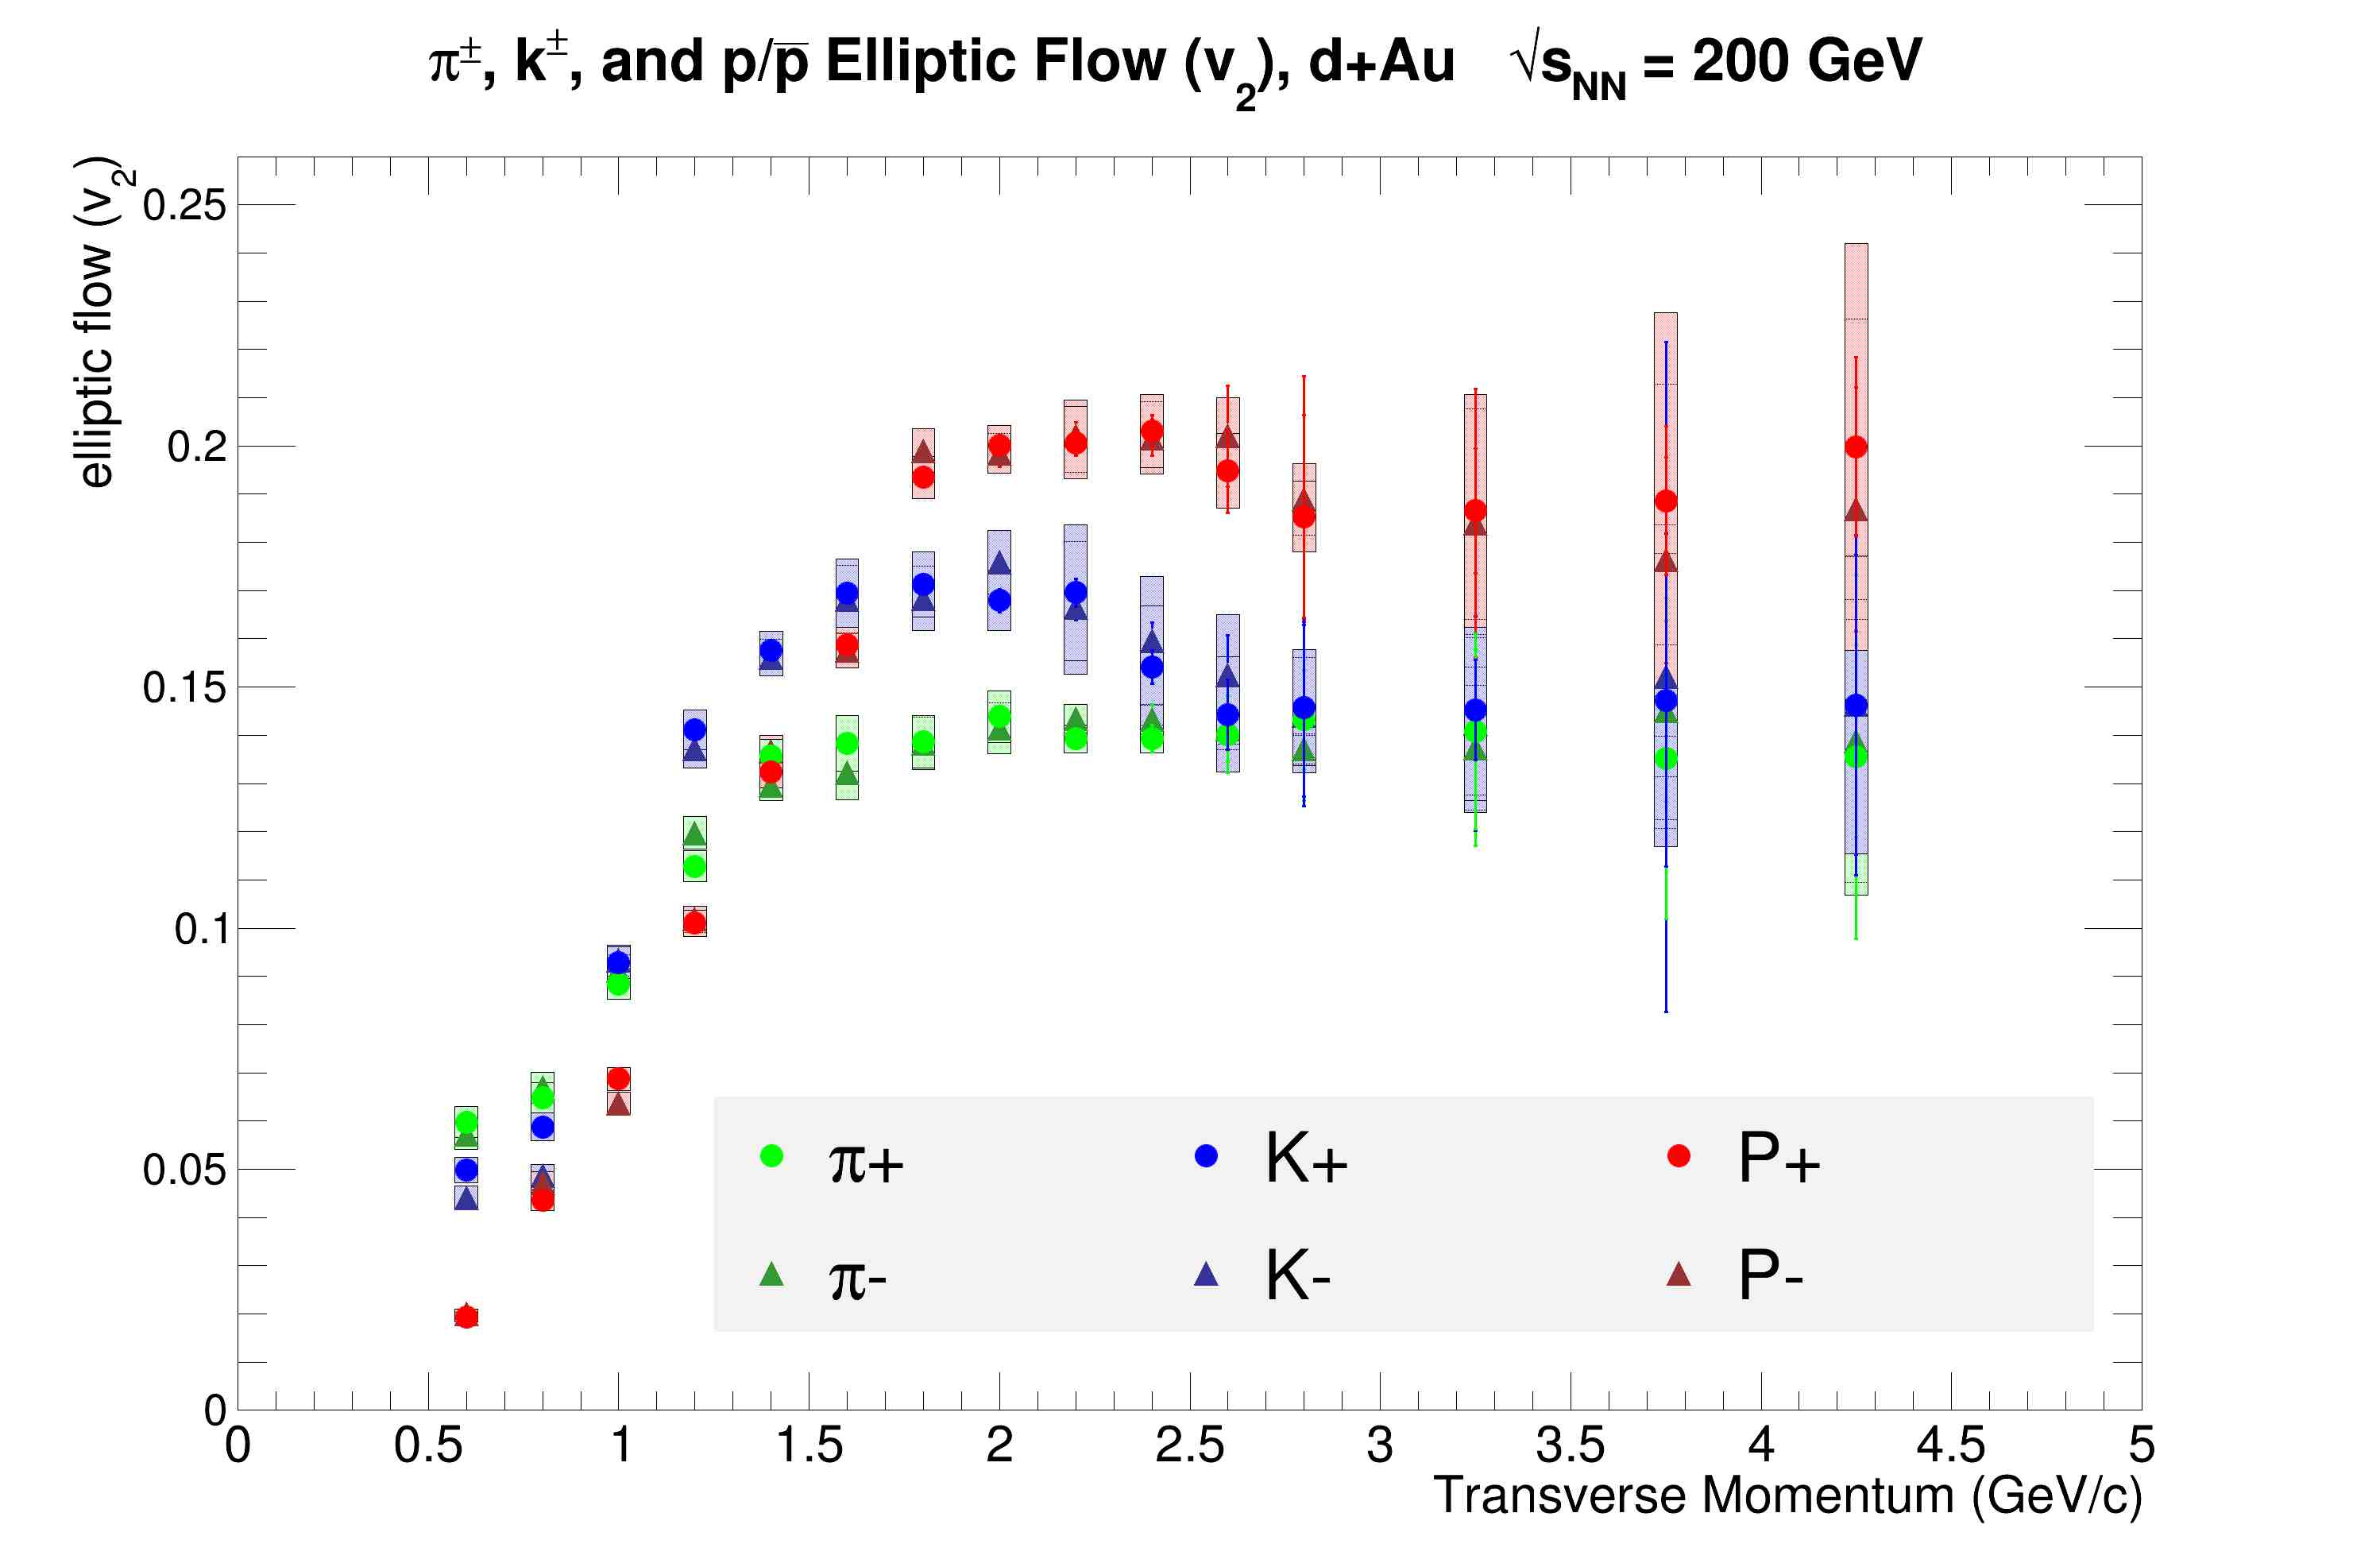
\includegraphics[width=0.7\textwidth]{results/v2all.jpg}
    \rule{35em}{0.5pt}
    \caption[Elliptic Flow vs Transverse Momentum, 200 GeV d+Au, 0-5\% centrality]{Elliptic Flow vs Transverse Momentum, 200 GeV d+Au, 0-5\% centrality}
    \label{fig:v2main}
\end{figure}

Measurements of the second Fourier coefficient corresponding to an elliptically shaped azimuthal anisotropy of pions, kaons, and (anti)protons produced in 200 GeV deuteron-gold collisions are presented in figure \ref{fig:v2main}. Historically, a large number of participant nucleons was thought to be required to be needed in order to produce a QGP. Consequently, it was thought that the low number of participant nucleons in the d+Au system was insufficient for such a phase change. The nonzero flow measurement in this analysis is a sign that collective behavior happens in systems previously thought of as ``cold'' and is an indication that a QGP could be formed in the simpler system of d+Au. This flow increases steadily for all hadrons up to $p_T \sim 1.5 $ GeV/c where the mesons (pions and kaons) seem to reach a saturation and flatten out. The kaons exhibit a flow signal stronger than the pions in this range but eventually decrease to the same nominal value as the pions. The (anti)protons continue to flow increasingly up to $p_T \sim 2$ GeV/c where they too flatten out. The measurement of particles and their corresponding antiparticles was separated throughout the course of the analysis. In doing so, flow coefficients for negative and positive charged particles for a given species can be compared. Here we see that the collision, evolution, and freeze out of the d+Au system does not favor particles or antiparticles, as expected.

\section{Discussion}

\subsection{Hadronization}
\begin{figure}[hbtp]
\centering    
    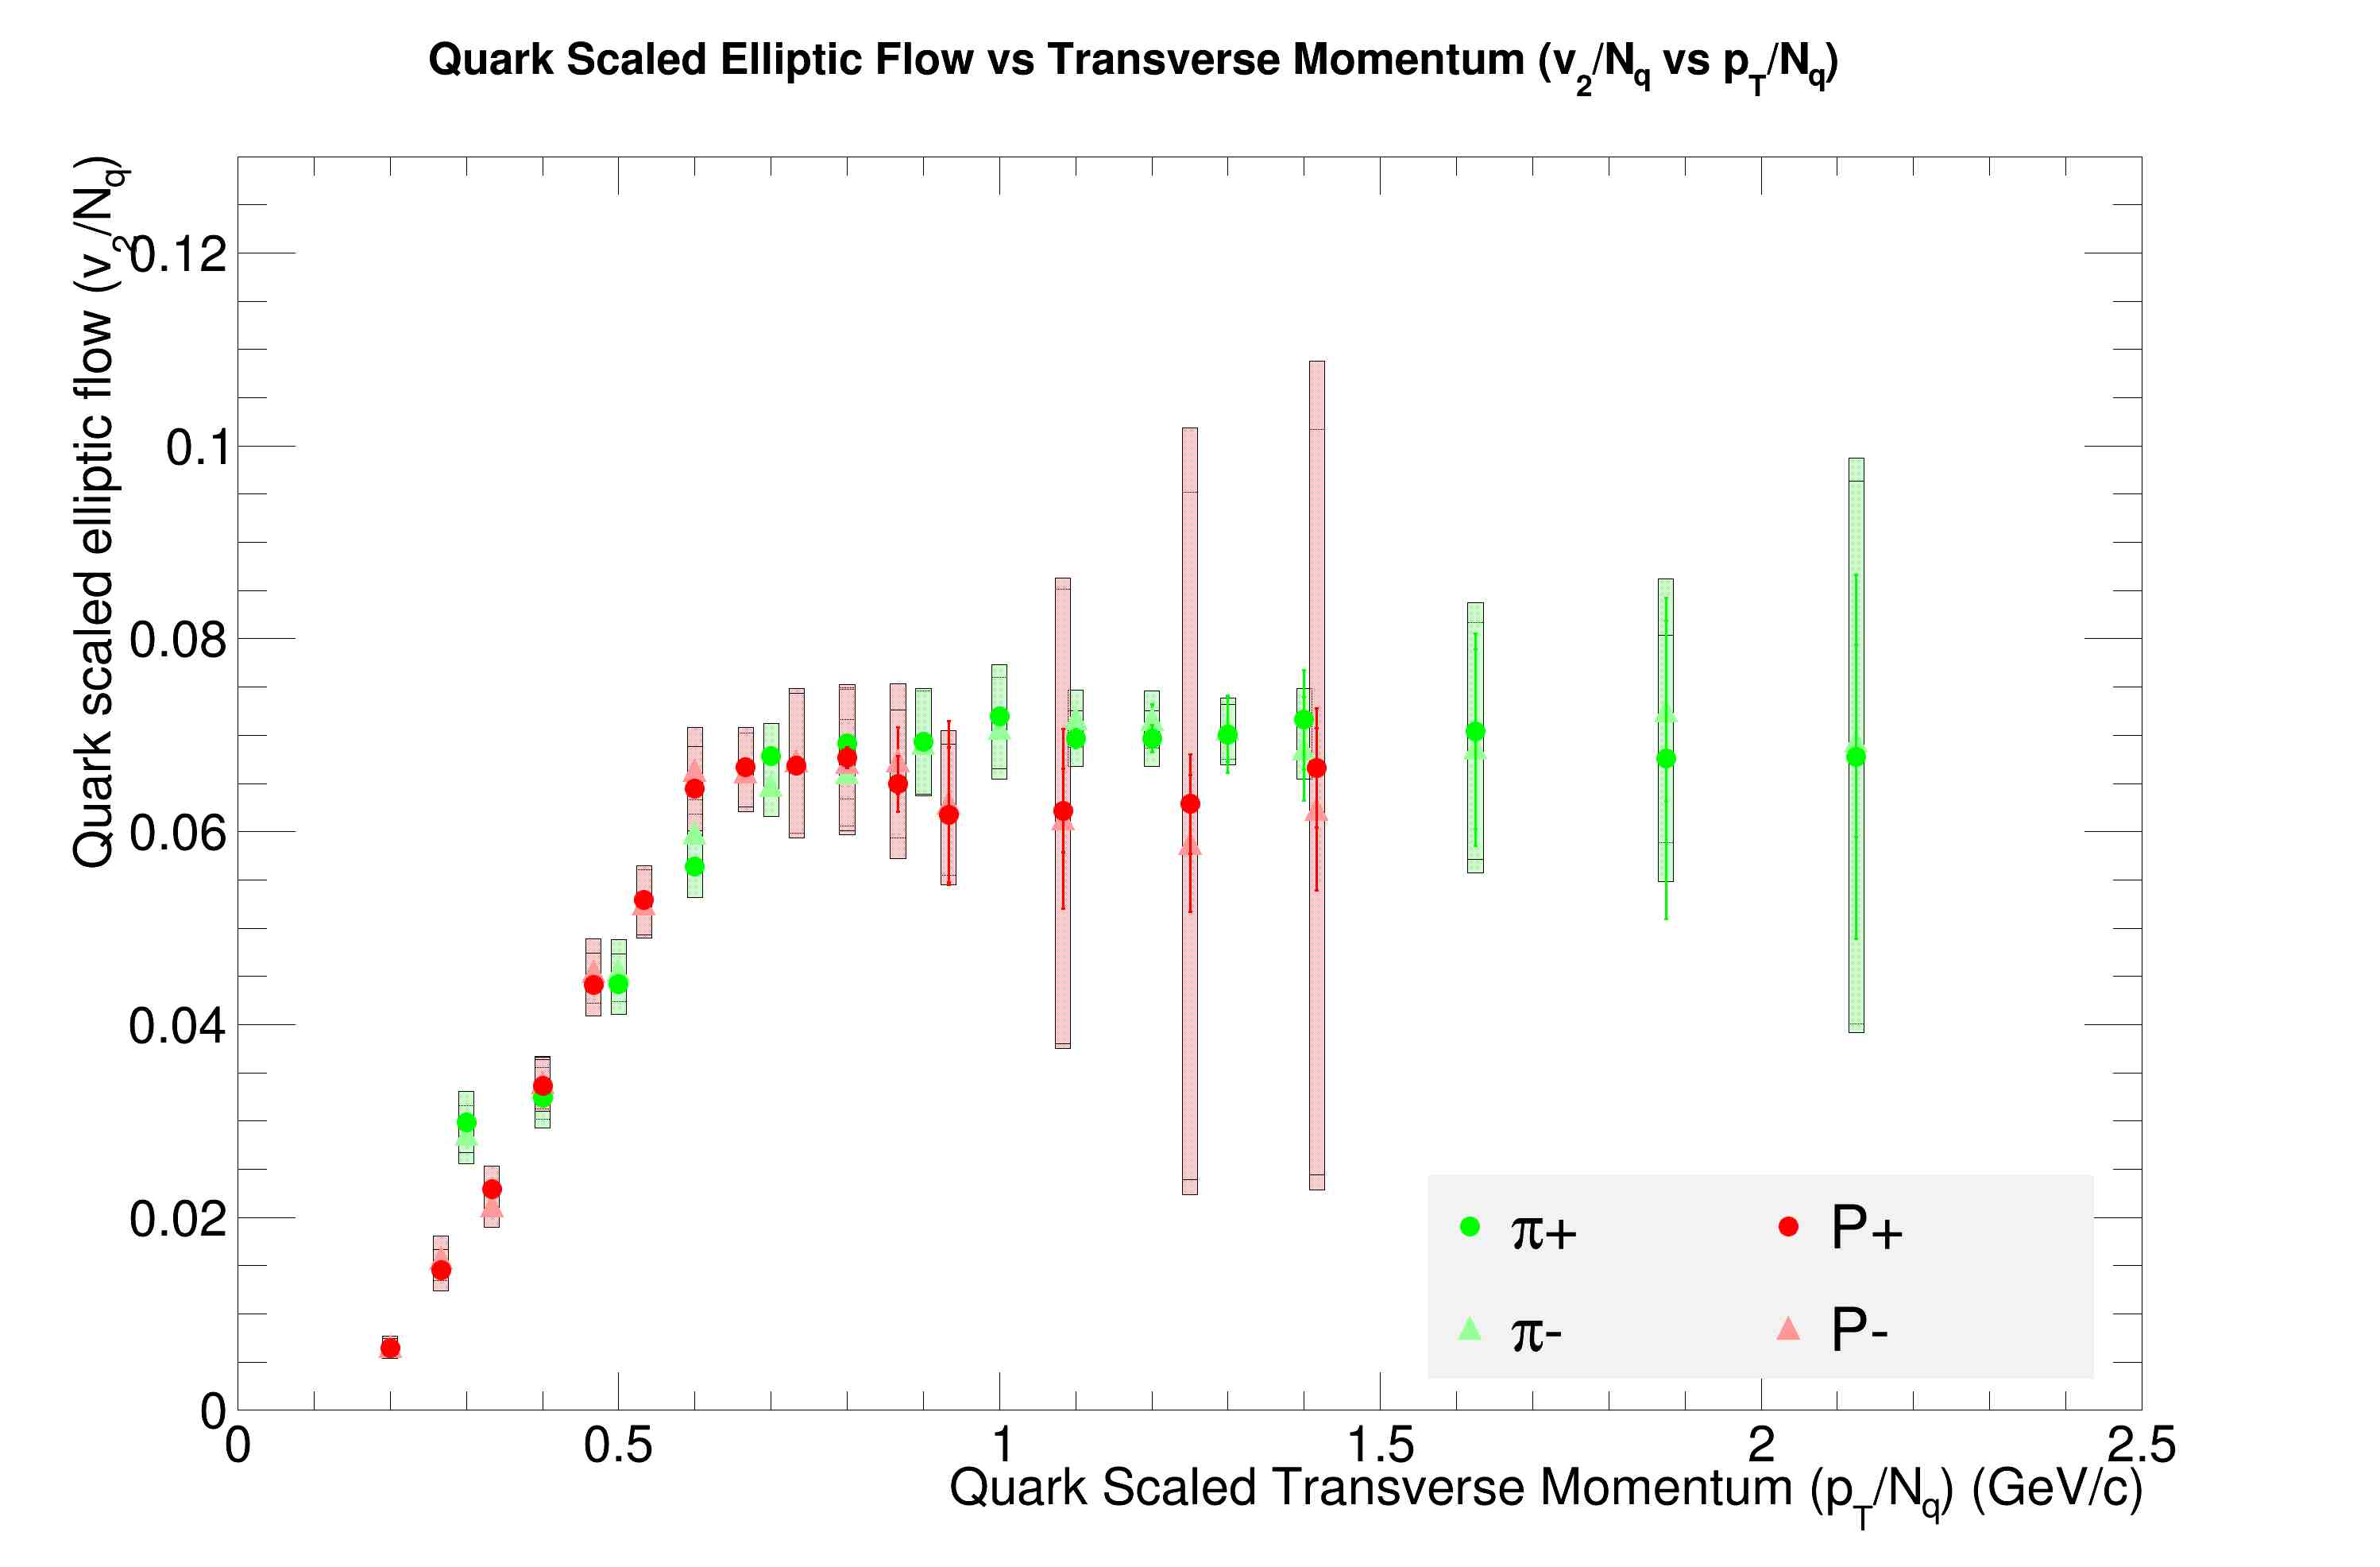
\includegraphics[width=0.7\textwidth]{results/v2NqvspT.jpg}
    \rule{35em}{0.5pt}
    \caption[Quark Scaled Elliptic Flow ($\pi^{\pm}$ and $p/\bar{p}$) vs Transverse Momentum, 200 GeV d+Au]{Quark Scaled Elliptic Flow ($\pi^{\pm}$ and $p/\bar{p}$) vs Transverse Momentum, 200 GeV d+Au}
    \label{fig:qscaledv2}
\end{figure}

The (anti)proton flow enhancement in the mid-$p_T$ range is similar to the baryon enhancement seen in previous experiments and the observation of collective flow is a strong indication of quark deconfinement/QGP formation. Because of this deconfinement, baryon enhancement must happen with some mechanism in the freeze out stage. The leading model describing this phenomenon, recombination, can be seen by scaling the flow coefficient and momentum by the number of quarks that comprise the measured particle\footnote{2 quarks for pions/kaons, 3 quarks for protons}. Doing so shows that this particle momentum discrepancy may come from the sum of momenta of the constituent quarks. That is to say, the reason why protons appear to have stronger flow is simply because they contain more quarks. For example, if we were to take three deconfined quarks that have the same momentum, they would hadronize to produce a particle with higher momentum than if only two of those quarks had combined. This quark scaled flow is shown in figure \ref{fig:qscaledv2} for pions and protons and shows that both particle signals increase and reach saturation in the same range. That the two quark scaled measurements track each other well through the $p_T$ range is a strong indication of recombination as the mechanism for thermal freeze-out and is a result that agrees with similar quark scaled results in $^3$He+Au\citep{huangQM2015}, Au+Au\citep{Adler:2003kt}, Cu+Cu\citep{PhysRevC.92.034913}, Pb+Pb\citep{Noferini:2012ps} systems both at RHIC and abroad.

\subsection{Comparison to Flow Models}
\begin{figure}[hbtp]
\centering    
    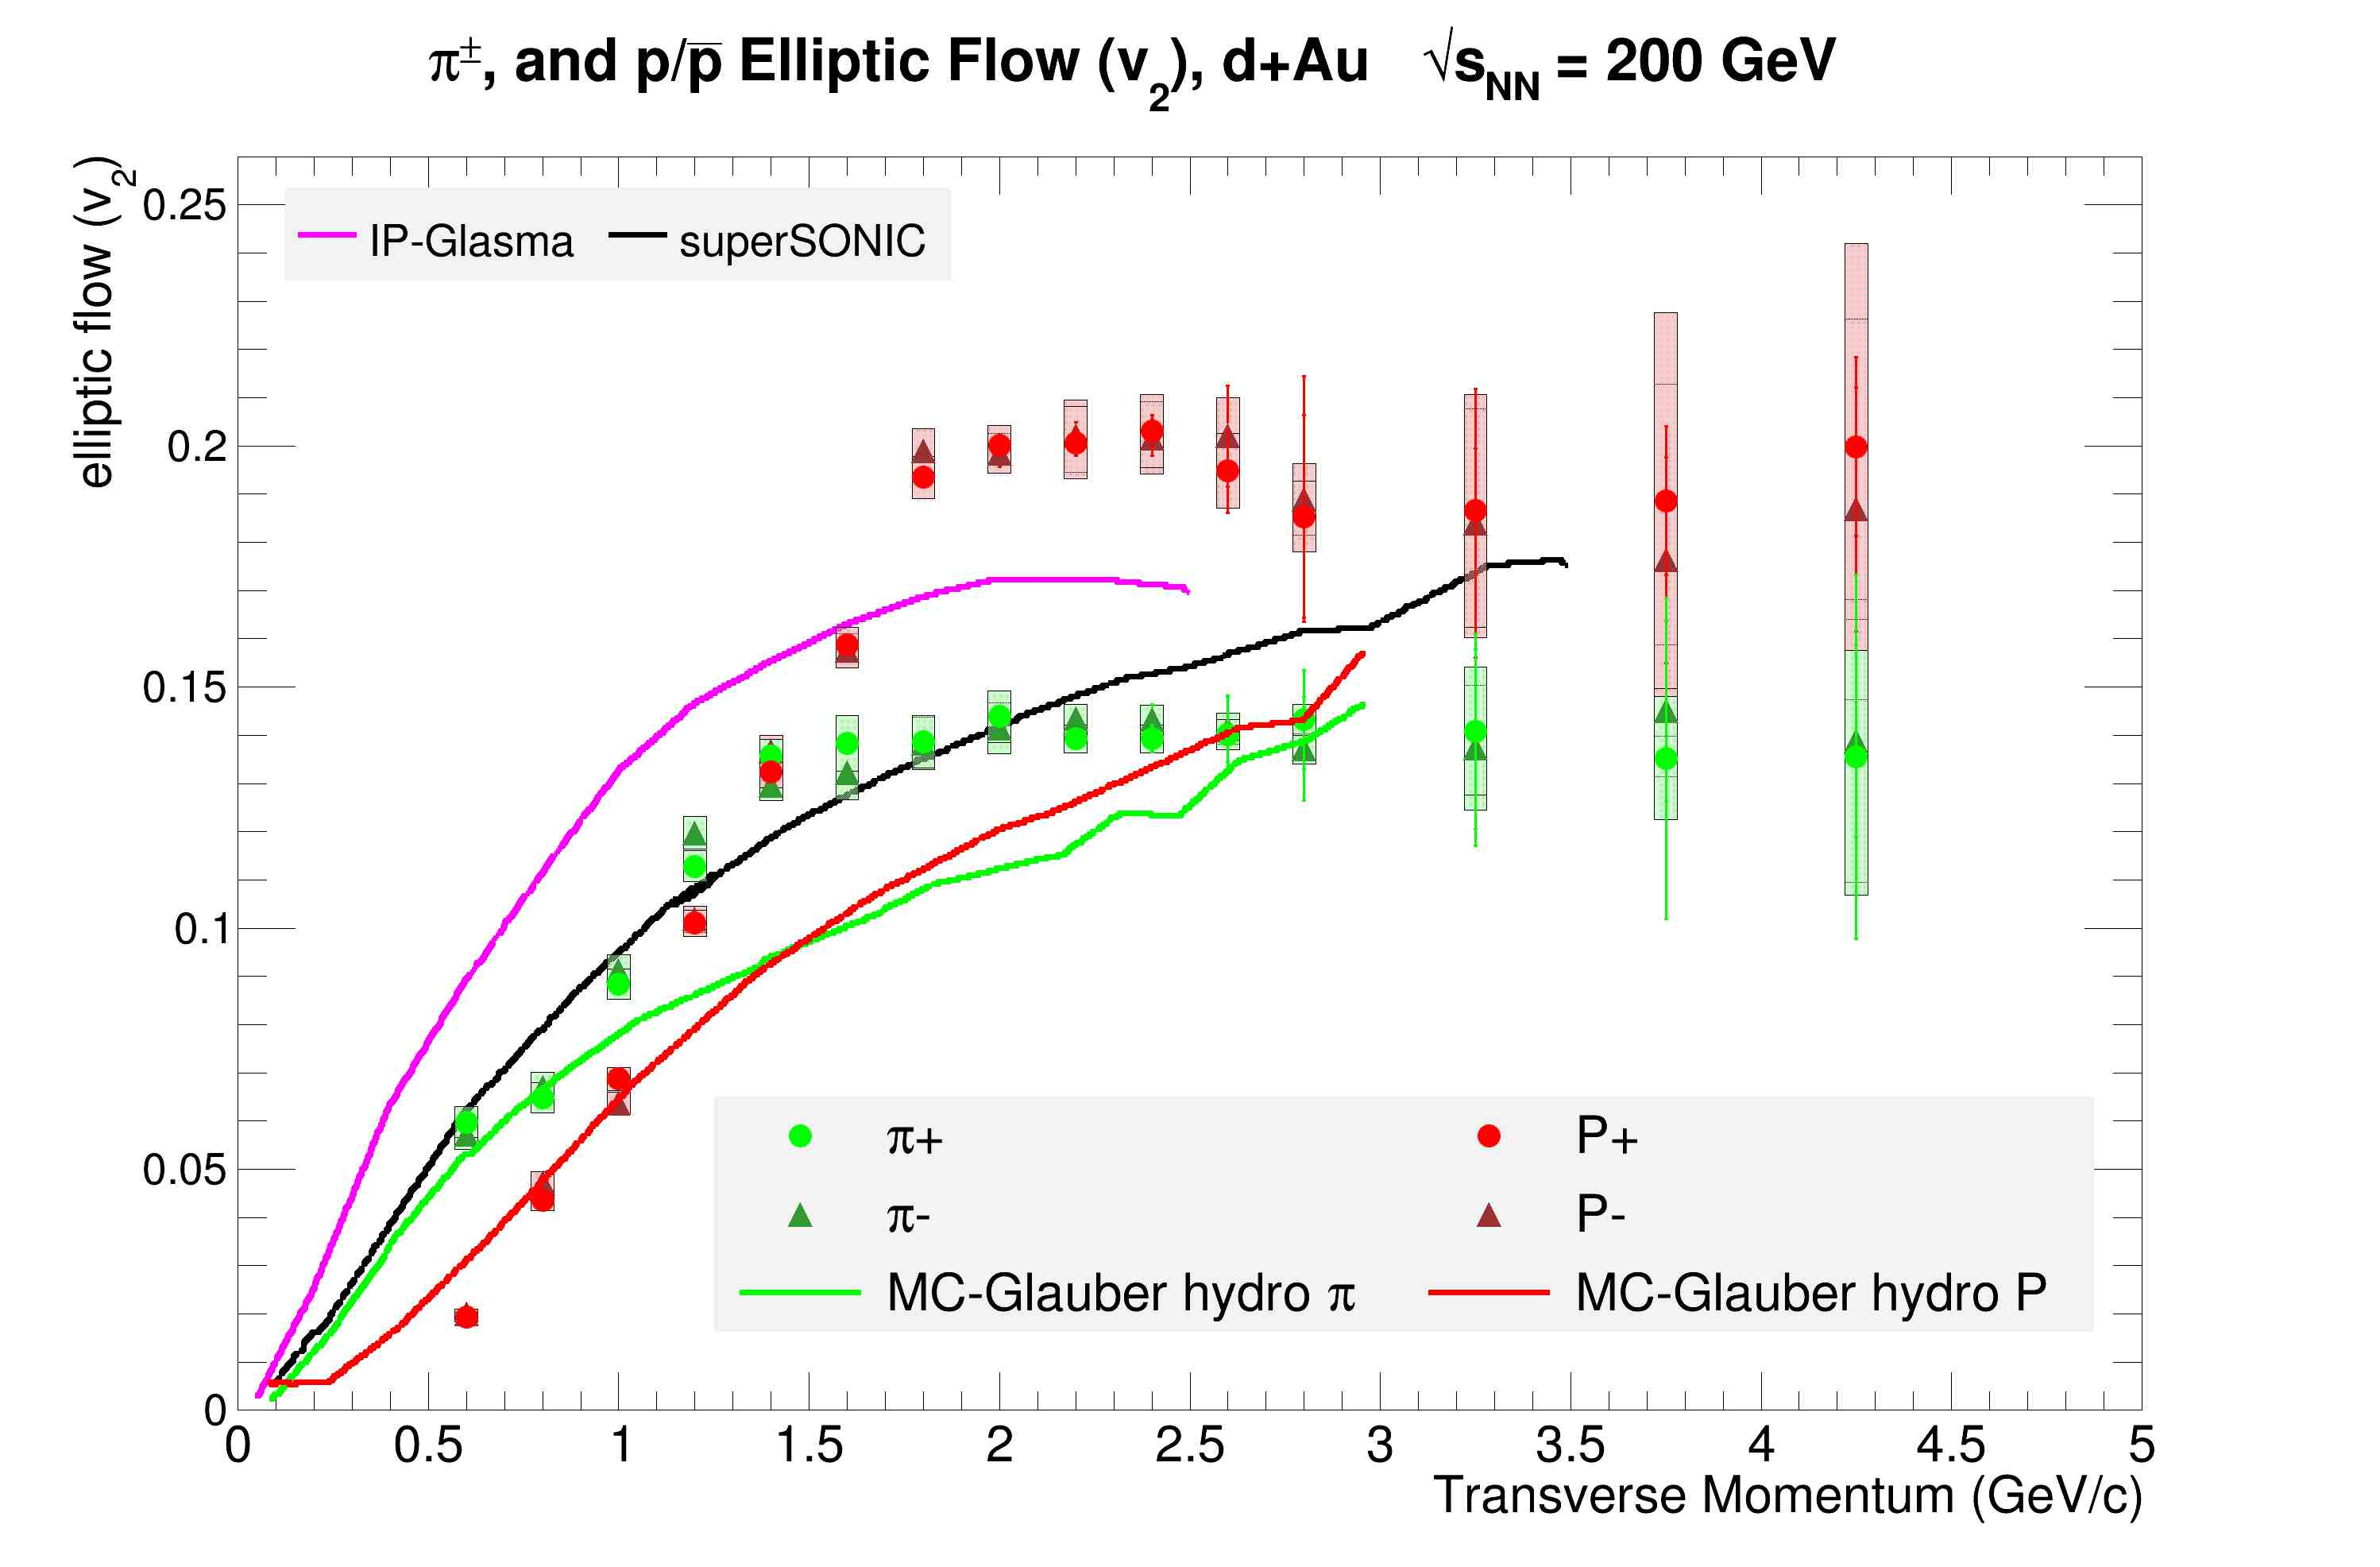
\includegraphics[width=0.5\textwidth]{results/v2allpipmodels.jpg}
    \rule{35em}{0.5pt}
    \caption[$\pi^{\pm}$ and $p/\bar{p}$ Elliptic Flow compared to hydrodynamic models.]{$\pi^{\pm}$ and $p/\bar{p}$ Elliptic Flow compared to hydrodynamic models: MC-Glauber\citep{Nagle:2013lja}, IP-Glasma\citep{Schenke:2014gaa}, and superSONIC\citep{Romatschke2015}}.
    \label{fig:hydrov2}
\end{figure}

Prior to hadronization, the equilibrated state of deconfined quarks has been described well with viscous hydrodynamic models. The way these models differ is in their assumption of the initial conditions (Glauber versus CGC) and length of equilibration time. A comparison of this measurement with these hydrodynamic models is shown in figure \ref{fig:hydrov2}. Models using Monte Carlo simulations of identified particle flow that utilize Glauber initial conditions (MC-Glauber) describe the data well for low $p_T$ but diverge above $p_T \sim 1$ GeV/c, also seen in d+Au in a previous PHENIX analysis\citep{Adare:2014keg}\footnote{though diverging at slightly higher transverse momentum, $p_T < 1.5 $GeV/c}. A continuation of MC-Glauber including a longer equilibration time (longer period of \textit{pre-flow} before a thermalized QGP flow) and the effect of post freeze-out hadron interaction\footnote{referred to in literature as \textit{Hadronic Cascade Afterburner}} called \textit{superSONIC}\citep{Romatschke2015}\footnote{an extension of an earlier SONIC model with a longer pre-flow time. SONIC stands for \textit{Super hybrid mOdel simulatioN for relativistic heavy-Ion Collisions}\citep{Romatschke2015}} matches data through mid $p_T$ but does not match the flow signal's saturation that begins just below $p_T \sim 2$ GeV/c, an effect also seen in the aforementioned PHENIX d+Au analysis. A model using an impact parameter independent CGC initial condition with a Glasma thermalization phase (IP-Glasma)\citep{Schenke:2014gaa} overestimates the flow strength at low $p_T$ but does appear to model the asymptotic flow behavior at mid-high $p_T$, albeit overestimating the value of that maximum flow value slightly. These two models can be seen compared to the overall flow in figure \ref{fig:allhadronhydro}. In order to minimize the effect of baryon enhancement in mid $p_T$, the elliptic flow of all hadrons is approximated by summing the yields of all identified tracks and performing a flow analysis. 

\begin{figure}[hbtp]
\centering    
    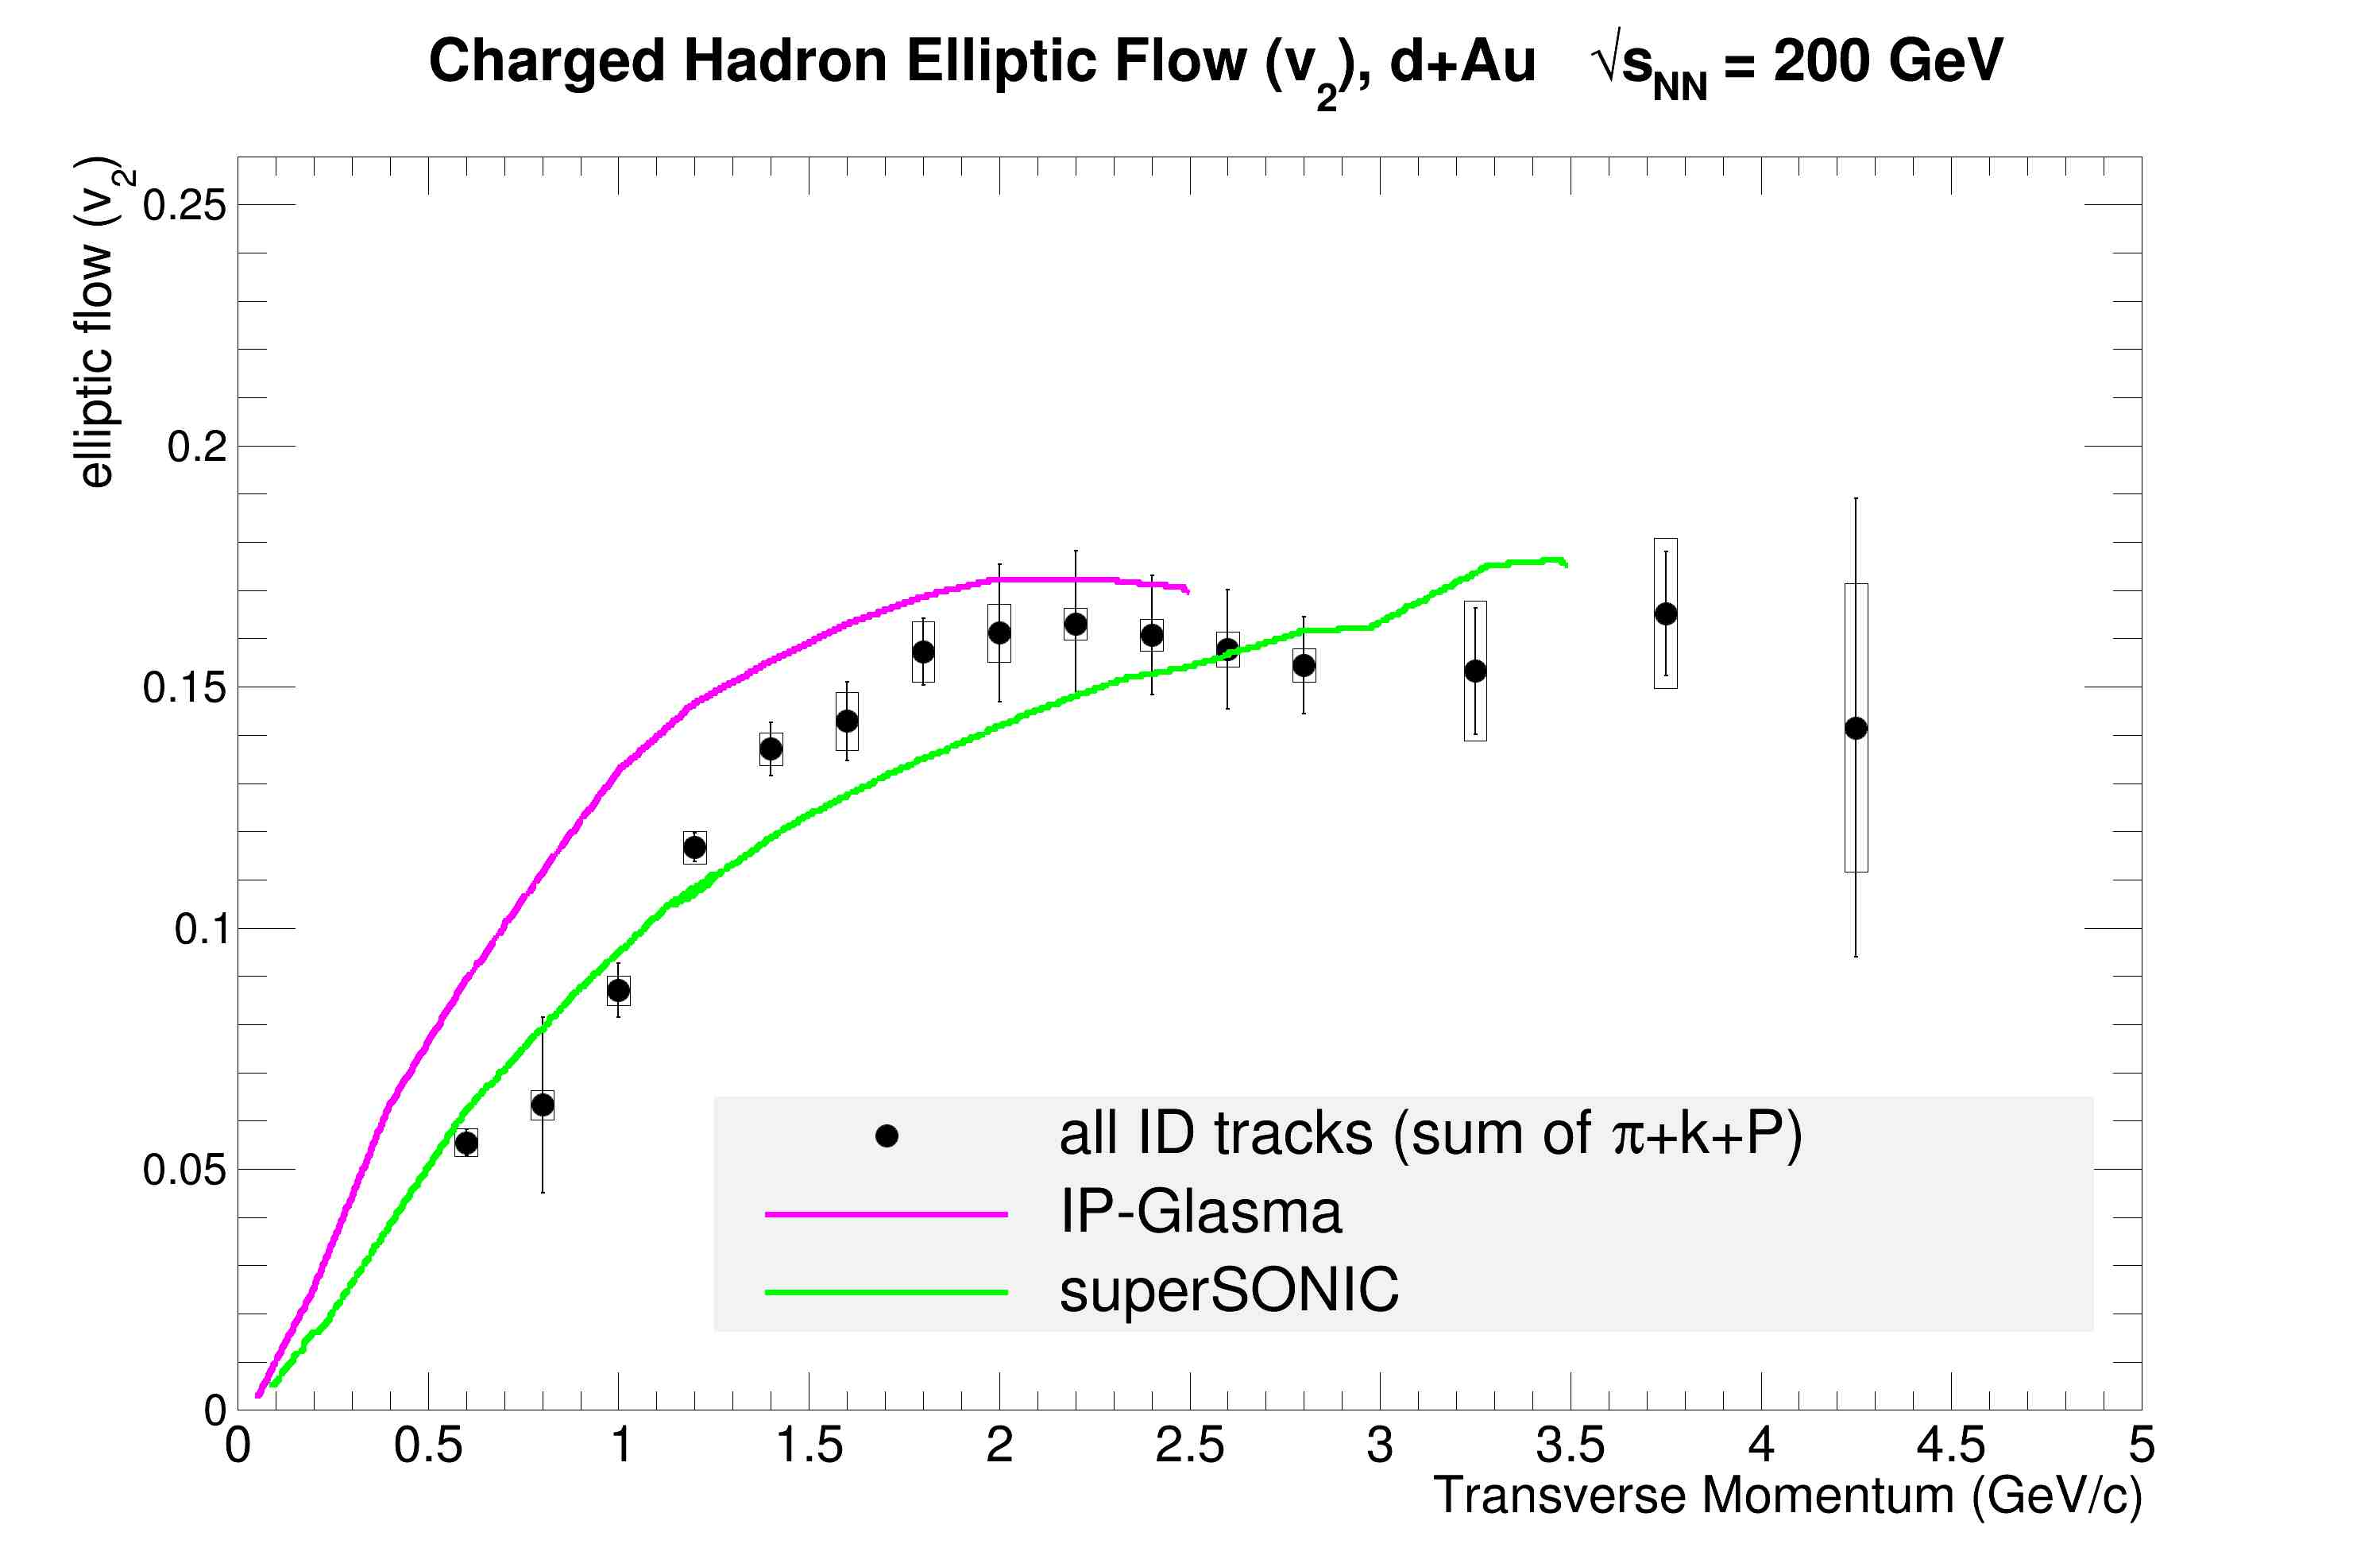
\includegraphics[width=0.5\textwidth]{results/v2hydro.jpg}
    \rule{35em}{0.5pt}
    \caption[Elliptic flow of all charged hadrons compared to hydrodynamic models.]{Elliptic flow of all charged hadrons measured by summing the yields of all identified tracks. Data is compared to IP-Glasma and superSONIC models.}
    \label{fig:allhadronhydro}
\end{figure}

\subsection{Strangeness and Initial Conditions}
While quark scaling can be used to explain pion and proton flow, implying that these hadrons are made by the combination of light flavor quarks, consistent with recombination, these quark building blocks had already existed before the collision in the form of valence quarks in the ions. What about strange quarks? These are created fresh from the collision, be it because of some process in thermalization\footnote{Glasma/pre-equilibrium flow}, or because of some strange quark producing mechanism in the flowing QGP\footnote{gluon fusion}. Previous enhancement was explained with a hadronization mechanism made evident by quark scaling protons and pions. However, this does not work for kaons as shown in figure \ref{fig:qscalemesonflow}. Here, the quark scaled kaon flow does not follow the flow of light flavor hadrons in the range $p_T \sim 0.7-1.3$ GeV/c, rather, it is stronger.

\begin{figure}[hbtp]
\centering
    \begin{subfigure}[h]{0.48\textwidth}
    \centering
    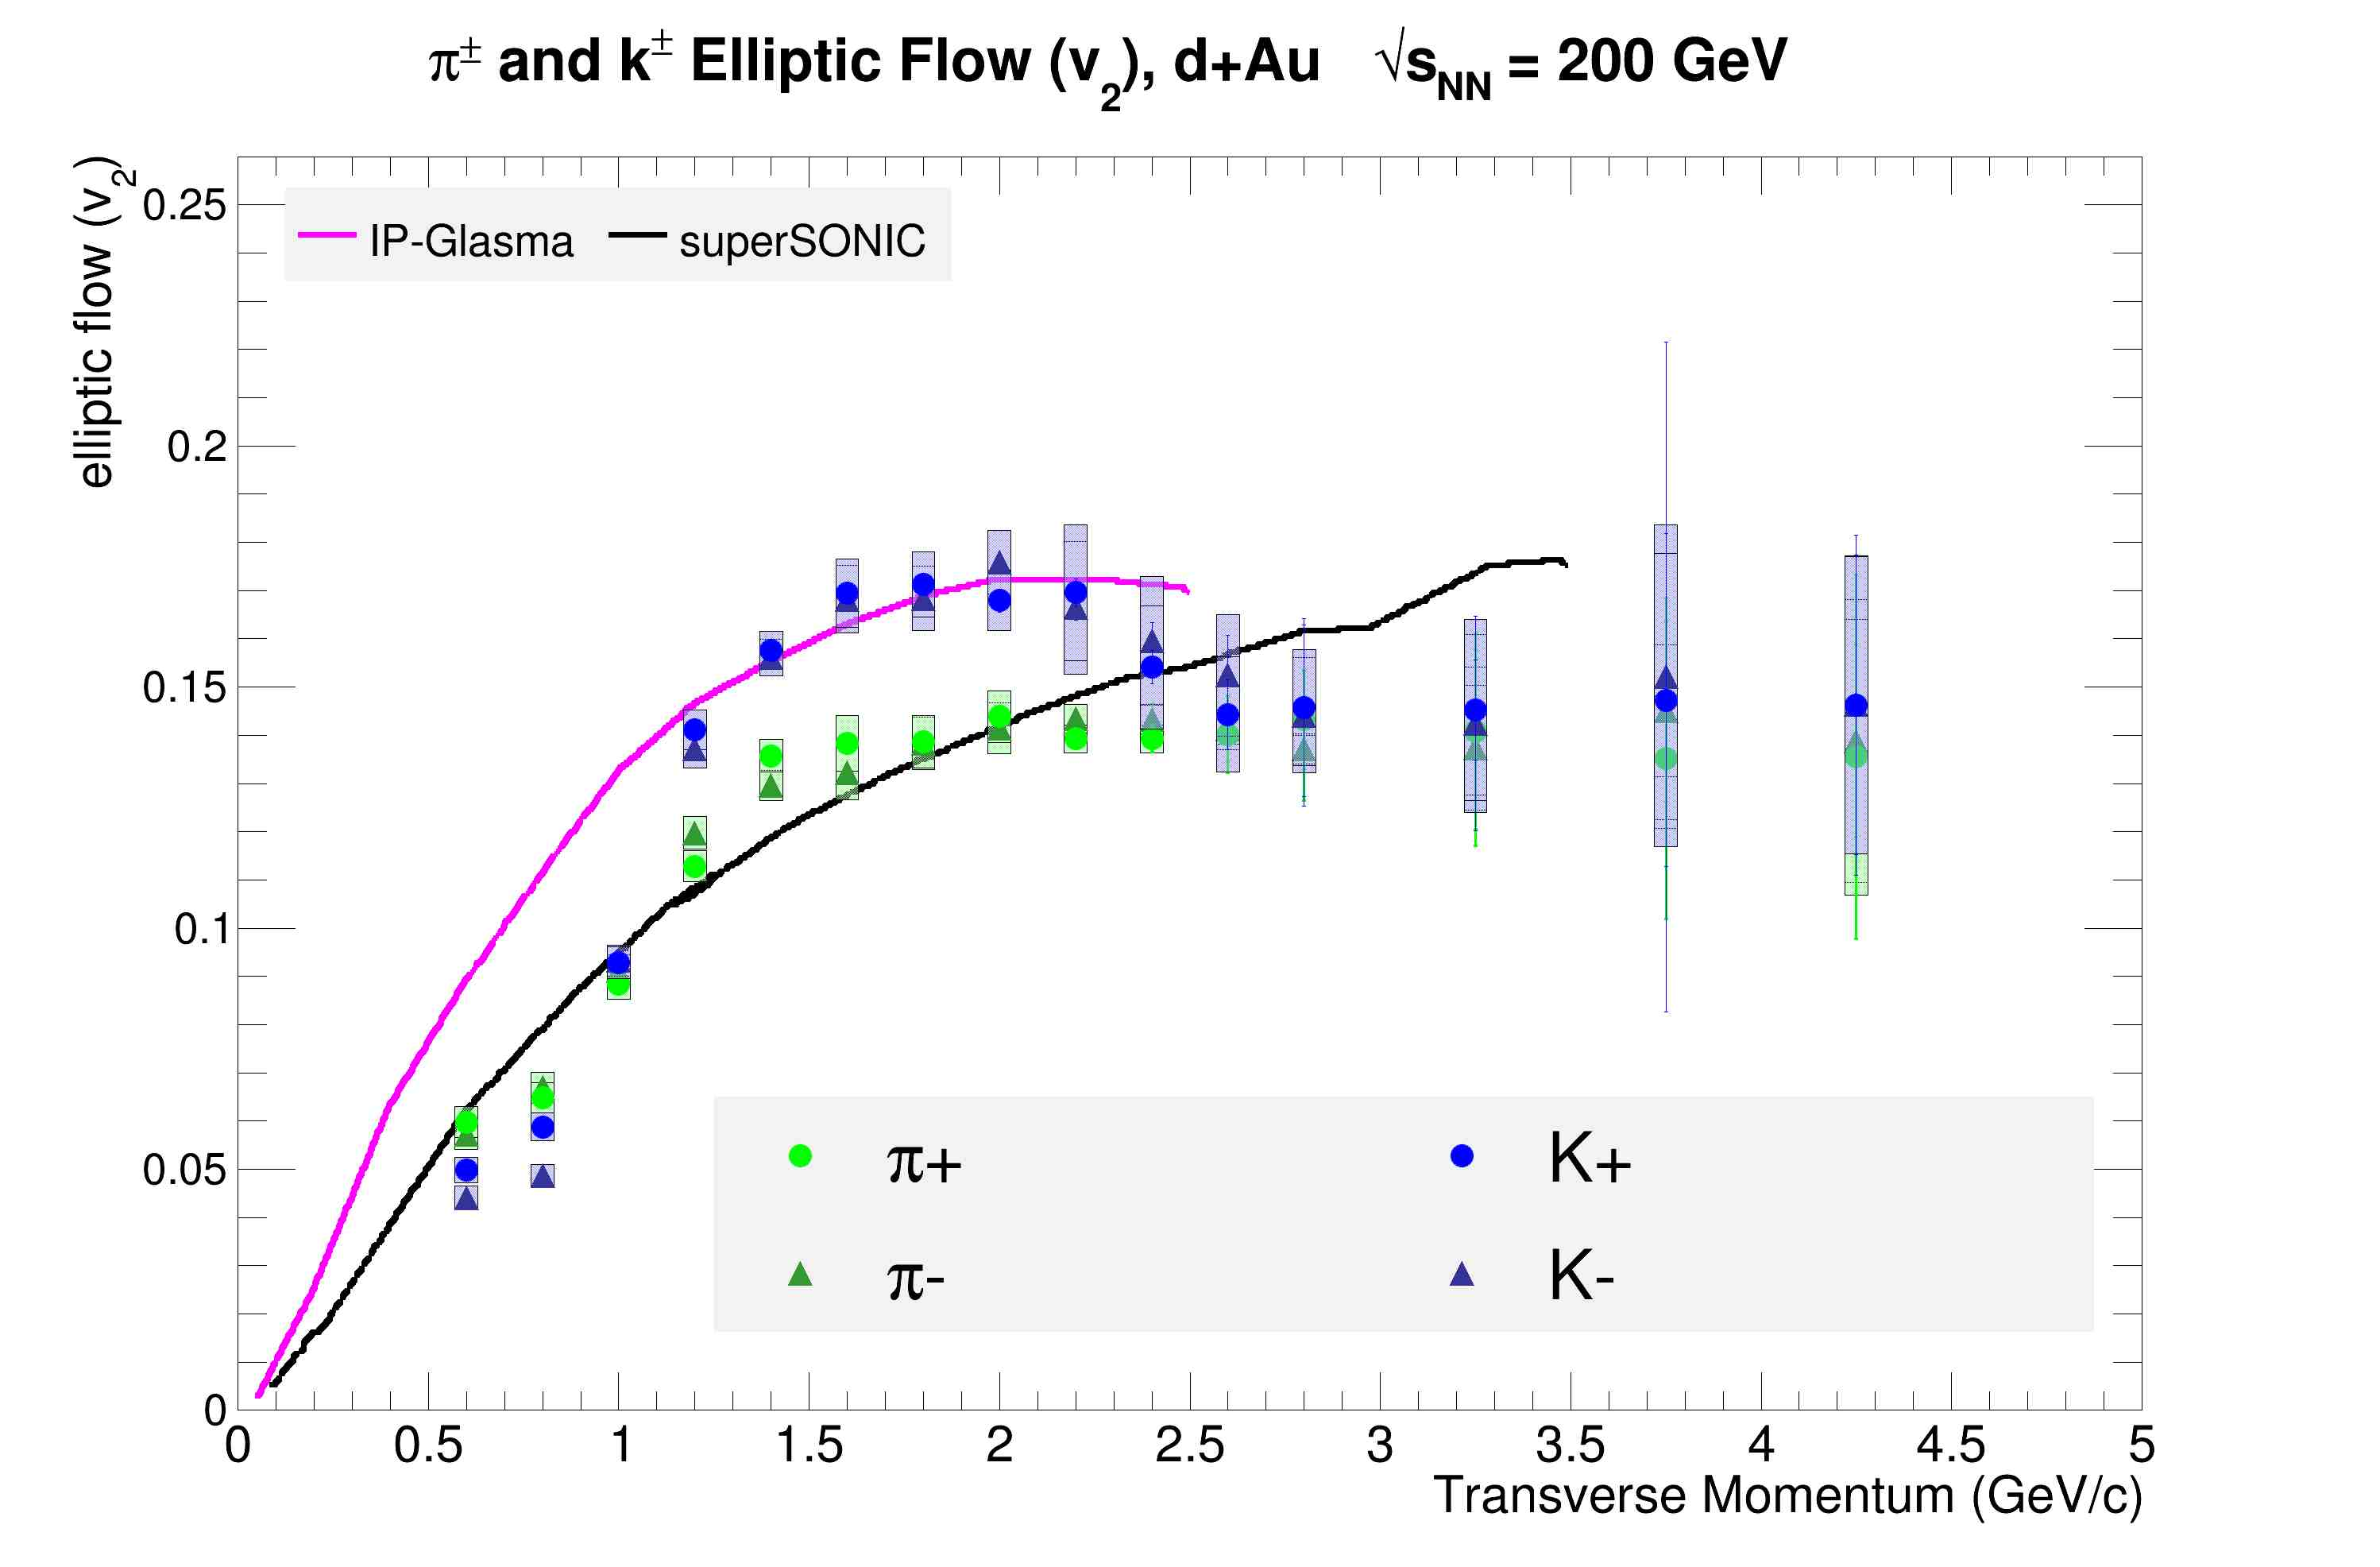
\includegraphics[width=1\textwidth]{results/v2mesons.jpg}

    \caption{Meson flow ($\pi^{\pm}$ and $K^{\pm}$).}
    \label{fig:smesonflow}
	\end{subfigure}
    \begin{subfigure}[h]{0.48\textwidth}
    \centering
    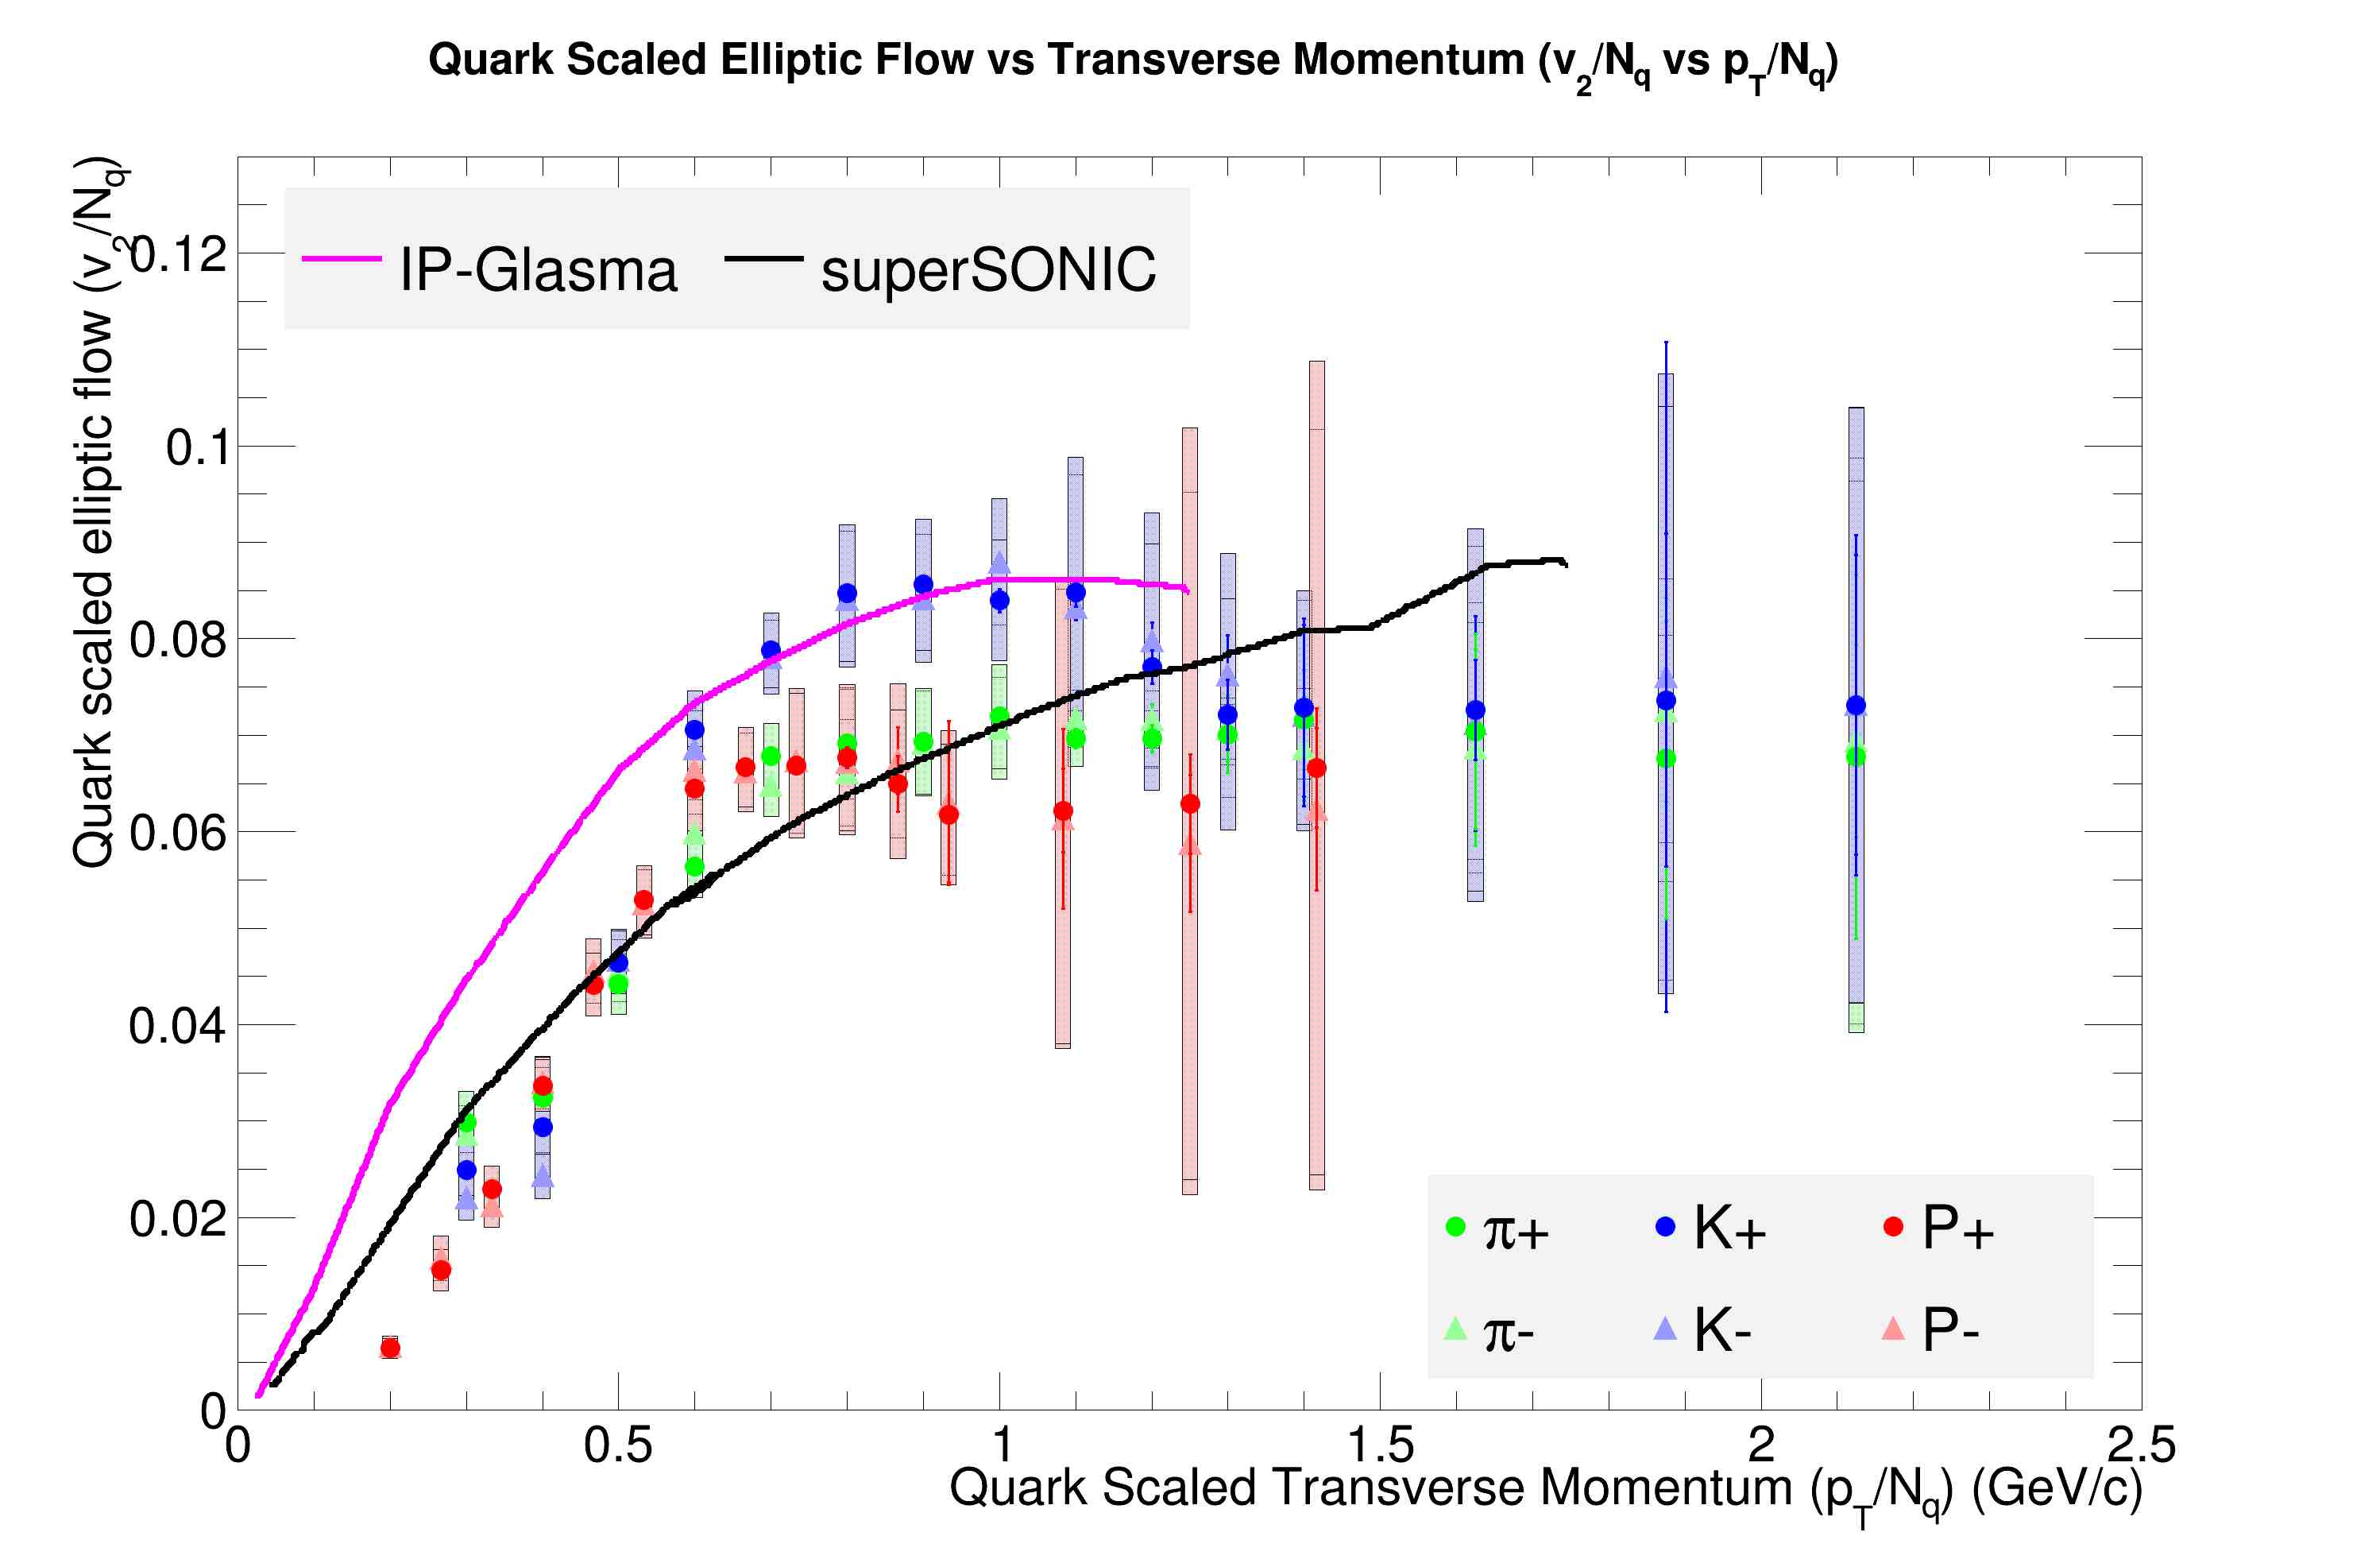
\includegraphics[width=1\textwidth]{results/v2NqvspTwmodels.jpg}
    \caption{Quark scaled elliptic flow ($\pi^{\pm}$,$K^{\pm}$,$p/\bar{p}$).}
    \label{fig:qscalemesonflow}

	\end{subfigure}
	\begin{subfigure}[h]{0.48\textwidth}
    \centering
    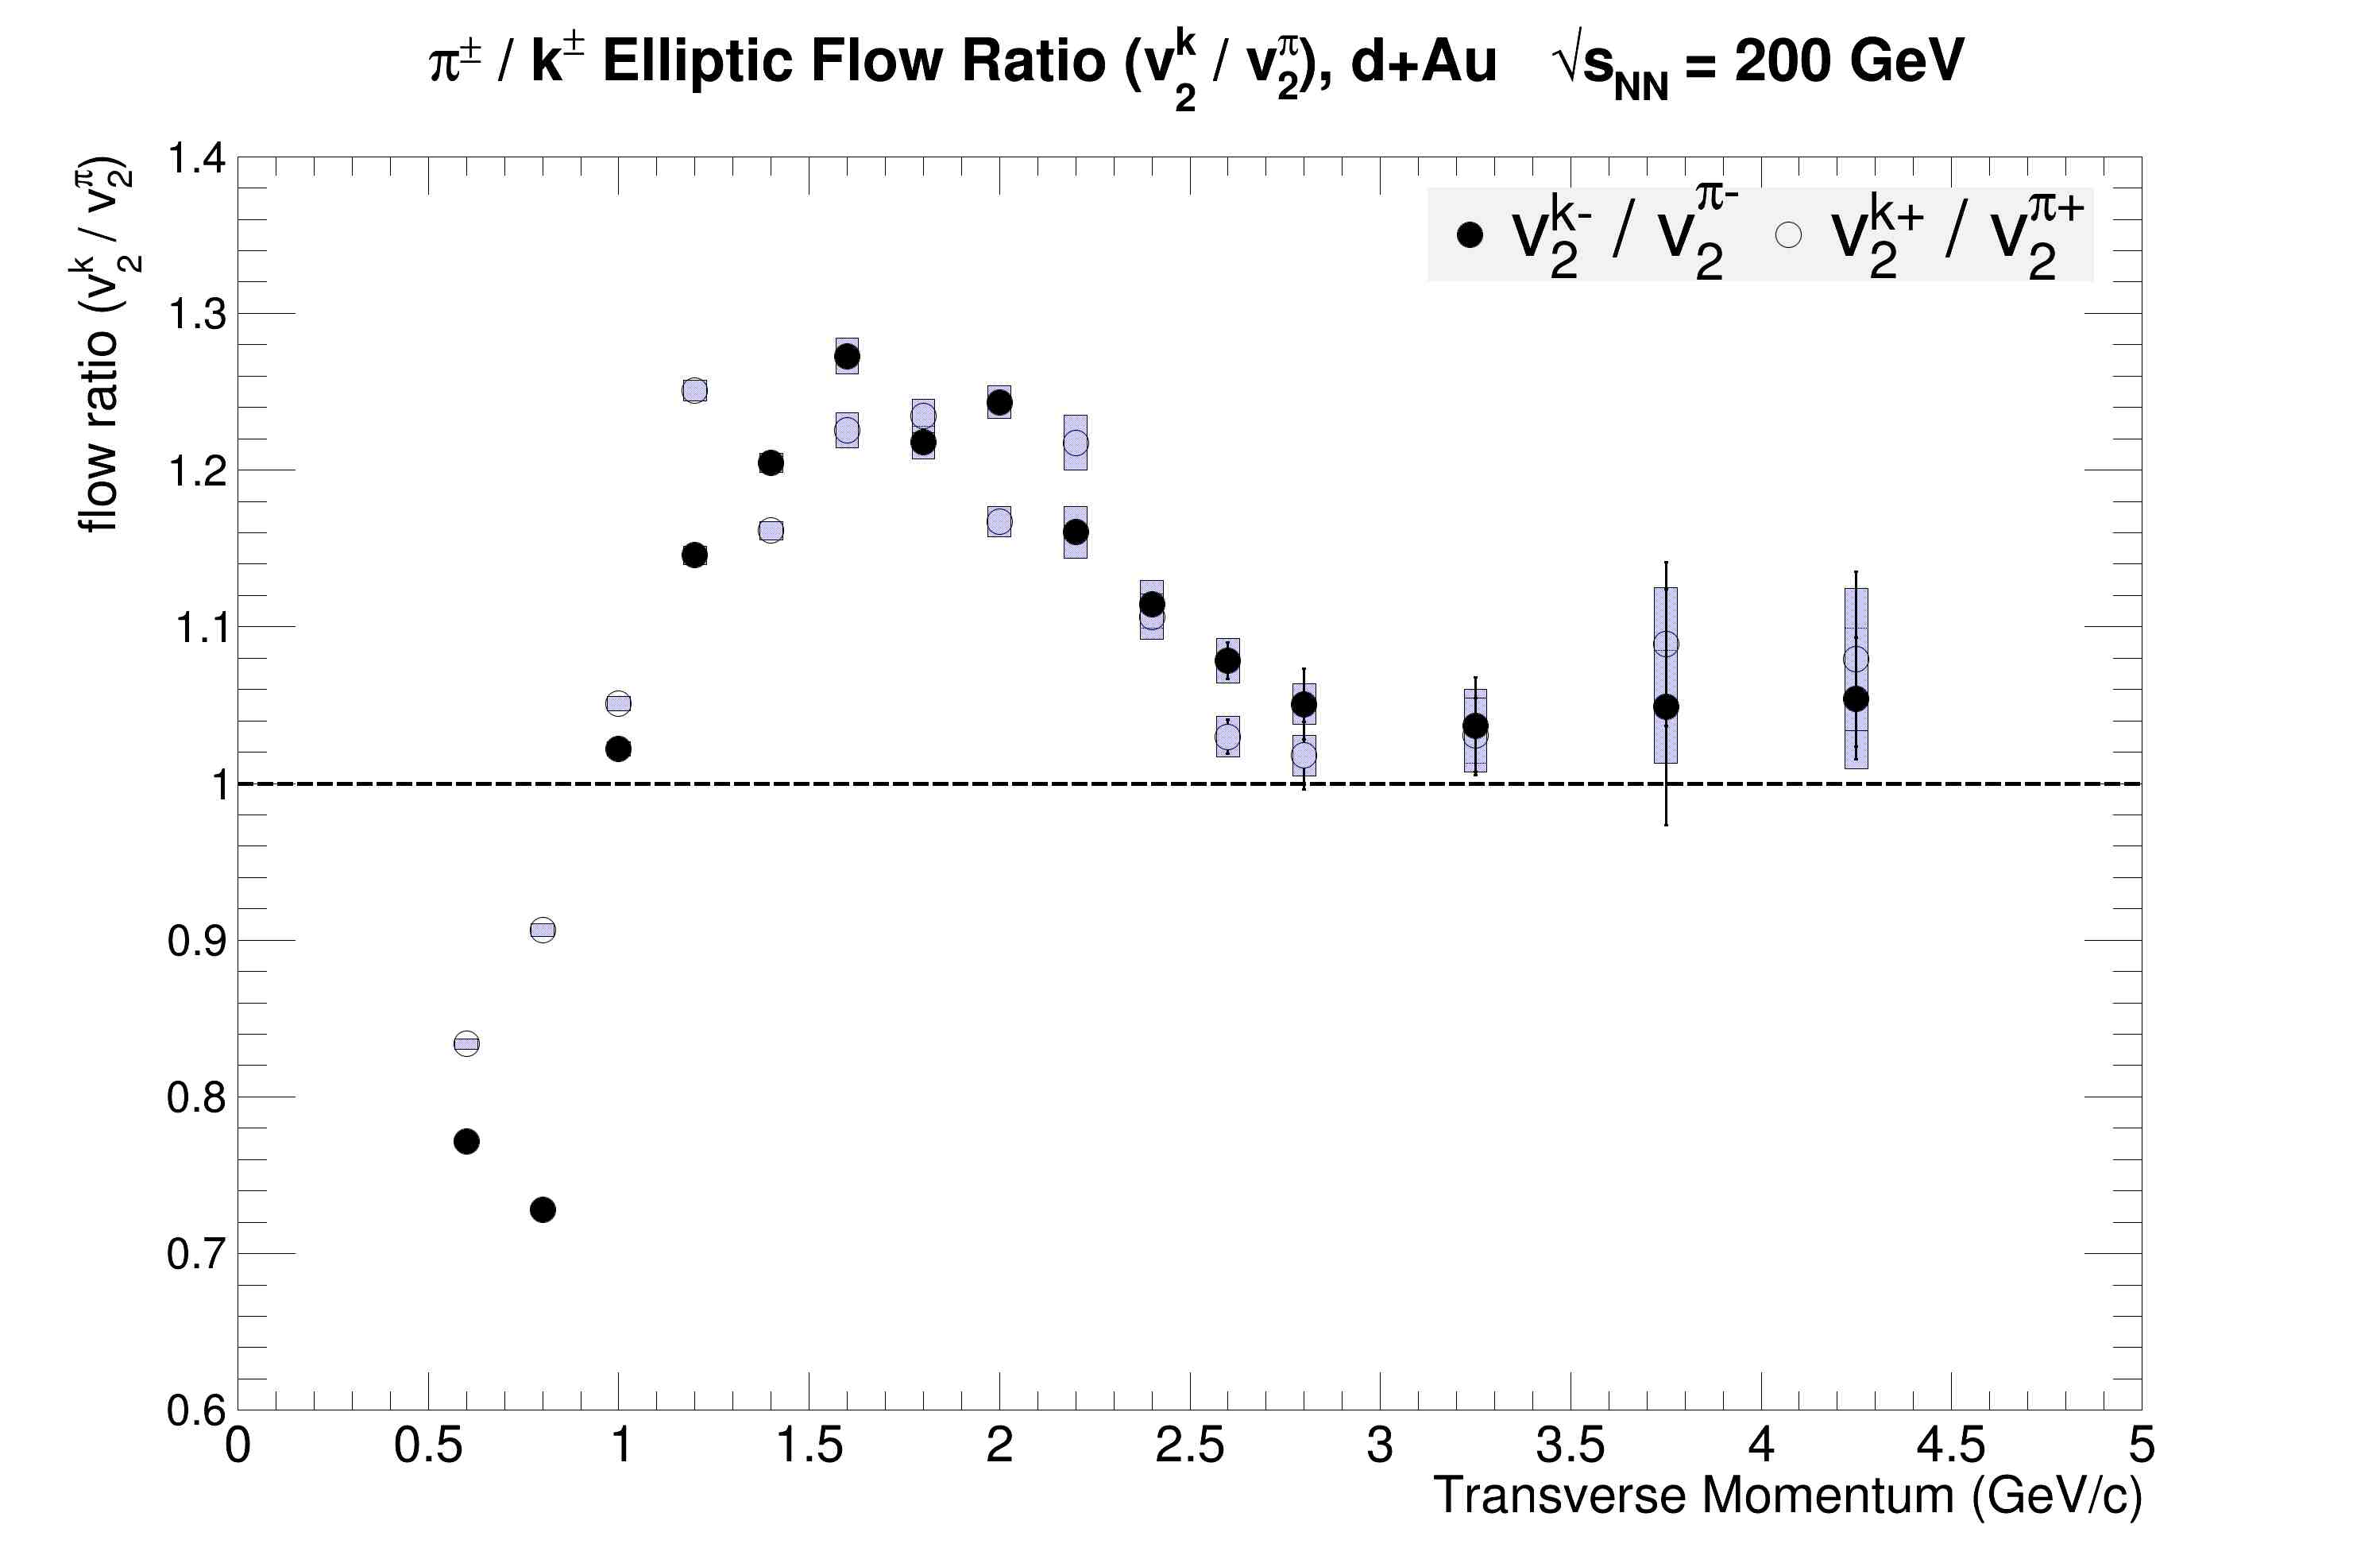
\includegraphics[width=1\textwidth]{results/v2mesonratio.jpg}
    \caption{Meson flow ratio ($v_2^{K} / v_2^{\pi}$).}
    \label{fig:mesonratio}

	\end{subfigure}

    \rule{35em}{0.5pt}
    \caption[Meson Elliptic Flow plots]{Elliptic flow of mesons ($\pi^{\pm}$ and $K^{\pm}$) are compared to hydrodynamic models. Where hadrons comprised from first generation quarks obey quark scaling, strange quark-containing kaons show an excess. CGC containing model seems to model kaon behavior at mid-$p_T$ well.}
    \label{fig:qscaledhydro}
\end{figure}

It is shown in figure \ref{fig:qscaledv2} that quark scaling the hadron flow causes light flavor hadron flow to line up. That is to say, it removes the apparent baryon excess by attributing this excess to recombination of two versus three quarks. However, we see that whatever mechanism creates strange quarks is not well described by Glauber initial conditions since there remains a stronger flow of strange quarks above the flow of light flavor quarks after quark scaling. In this range, the IP-Glasma model best fits the kaon flow (see fig. \ref{fig:smesonflow}). This implies that the choice of initial conditions and thermalization mechanisms in models may play a part in explaining strangeness enhancement and may be an indication of how CGC/Glasma may present itself in simple heavy ion systems. Following this thought, the Glauber model would be appropriate for describing light flavor quark flow since it treats the nucleus as a density function of these light quarks. The flow of light flavor hadrons is then described by the recombination and fragmentation of quarks that had already existed. On the other hand, the CGC initial condition has built within it a plethora of gluons due to low-x saturation. These gluons may generate flow in the pre-equilibrium stage\citep{Krasnitz200321}. Strangeness enhancement through gluon-gluon fusion has historically been proposed as a sign of the onset of QGP formation\citep{PhysRevLett.48.1066}, a phenomenon that combines well with the dominant availability of gluons in the CGC model. Similar strange flow enhancement above quark scaling has been seen in\footnote{in triangular flow ($v_3$) measured with $K^{\pm}$ and $\Lambda/\bar{\Lambda}$ compared to $\pi^{\pm}$ and $p/\bar{p}$.} Pb+Pb collisions\citep{1742-6596-668-1-012099} and at high kinetic energy in $^3$He+Au\citep{huangQM2015}. However, previous Au+Au results have shown that although kaon production appears to be enhanced \citep{Hohne:1999jf}, kaon flow seems to follow quark scaling. \citep{PhysRevC.92.034913} 

Furthermore, it may be advantageous to treat the flow of light flavor and heavy flavor quarks with different models. As mentioned, light quarks already existed and carry the majority of the momentum in the relativistic nucleus before collision. The time scale of these valence quarks makes them appear to move very fast compared to the saturated gluons, which may imply that the model describing the behavior of valence quarks is different from the model describing the behavior of the saturated gluons. We can therefore use the Glauber model as it was originally intended: as a description of quantum mechanical scattering for systems comprised of many particles (the light flavor quarks). 

On the other hand, the ``frustrated'' low-x gluons move much more slowly and may interact on different time scales than the valence quarks. Additionally, gluons do not exist on their own in nature, we can only detect what they hadronize into. Since heavy quarks are created fresh, they are a good candidate for a probe with which to study the interaction of low-x gluons.

\section{Comparison to Other Results}
Flow has been observed in other analyses of simple systems. Here I will compare my results to published results that analyzed other light-on-heavy ion collisions in order to see my results in the context of other measurements of the same phenomena . 

A previously published PHENIX analysis of $v_2$ in $\sqrt{s_{NN}}=$200 GeV d+Au collisions is shown in figure \ref{fig:v2allvsshengli}. The flow measurement here was calculated using two particle correlations\footnote{In contrast, my measurement uses a direct Fourier analysis of the flow.}. The two results track each other well in slope and strength of the flow up to $\sim$1.5 GeV/c and both reach saturation at $\sim$2.5 GeV/c. Both exhibit a crossover of the proton flow over the pion flow $\sim$1.5 GeV/c. I am able to measure in finer bins of $p_T$ since I use the ACC in conjunction with the TOF.W in order to maintain meson separation.  Furthermore, this allows me to study kaon flow, a measurement that this previous publication does not include.

\begin{figure}[hbtp]
\centering    
    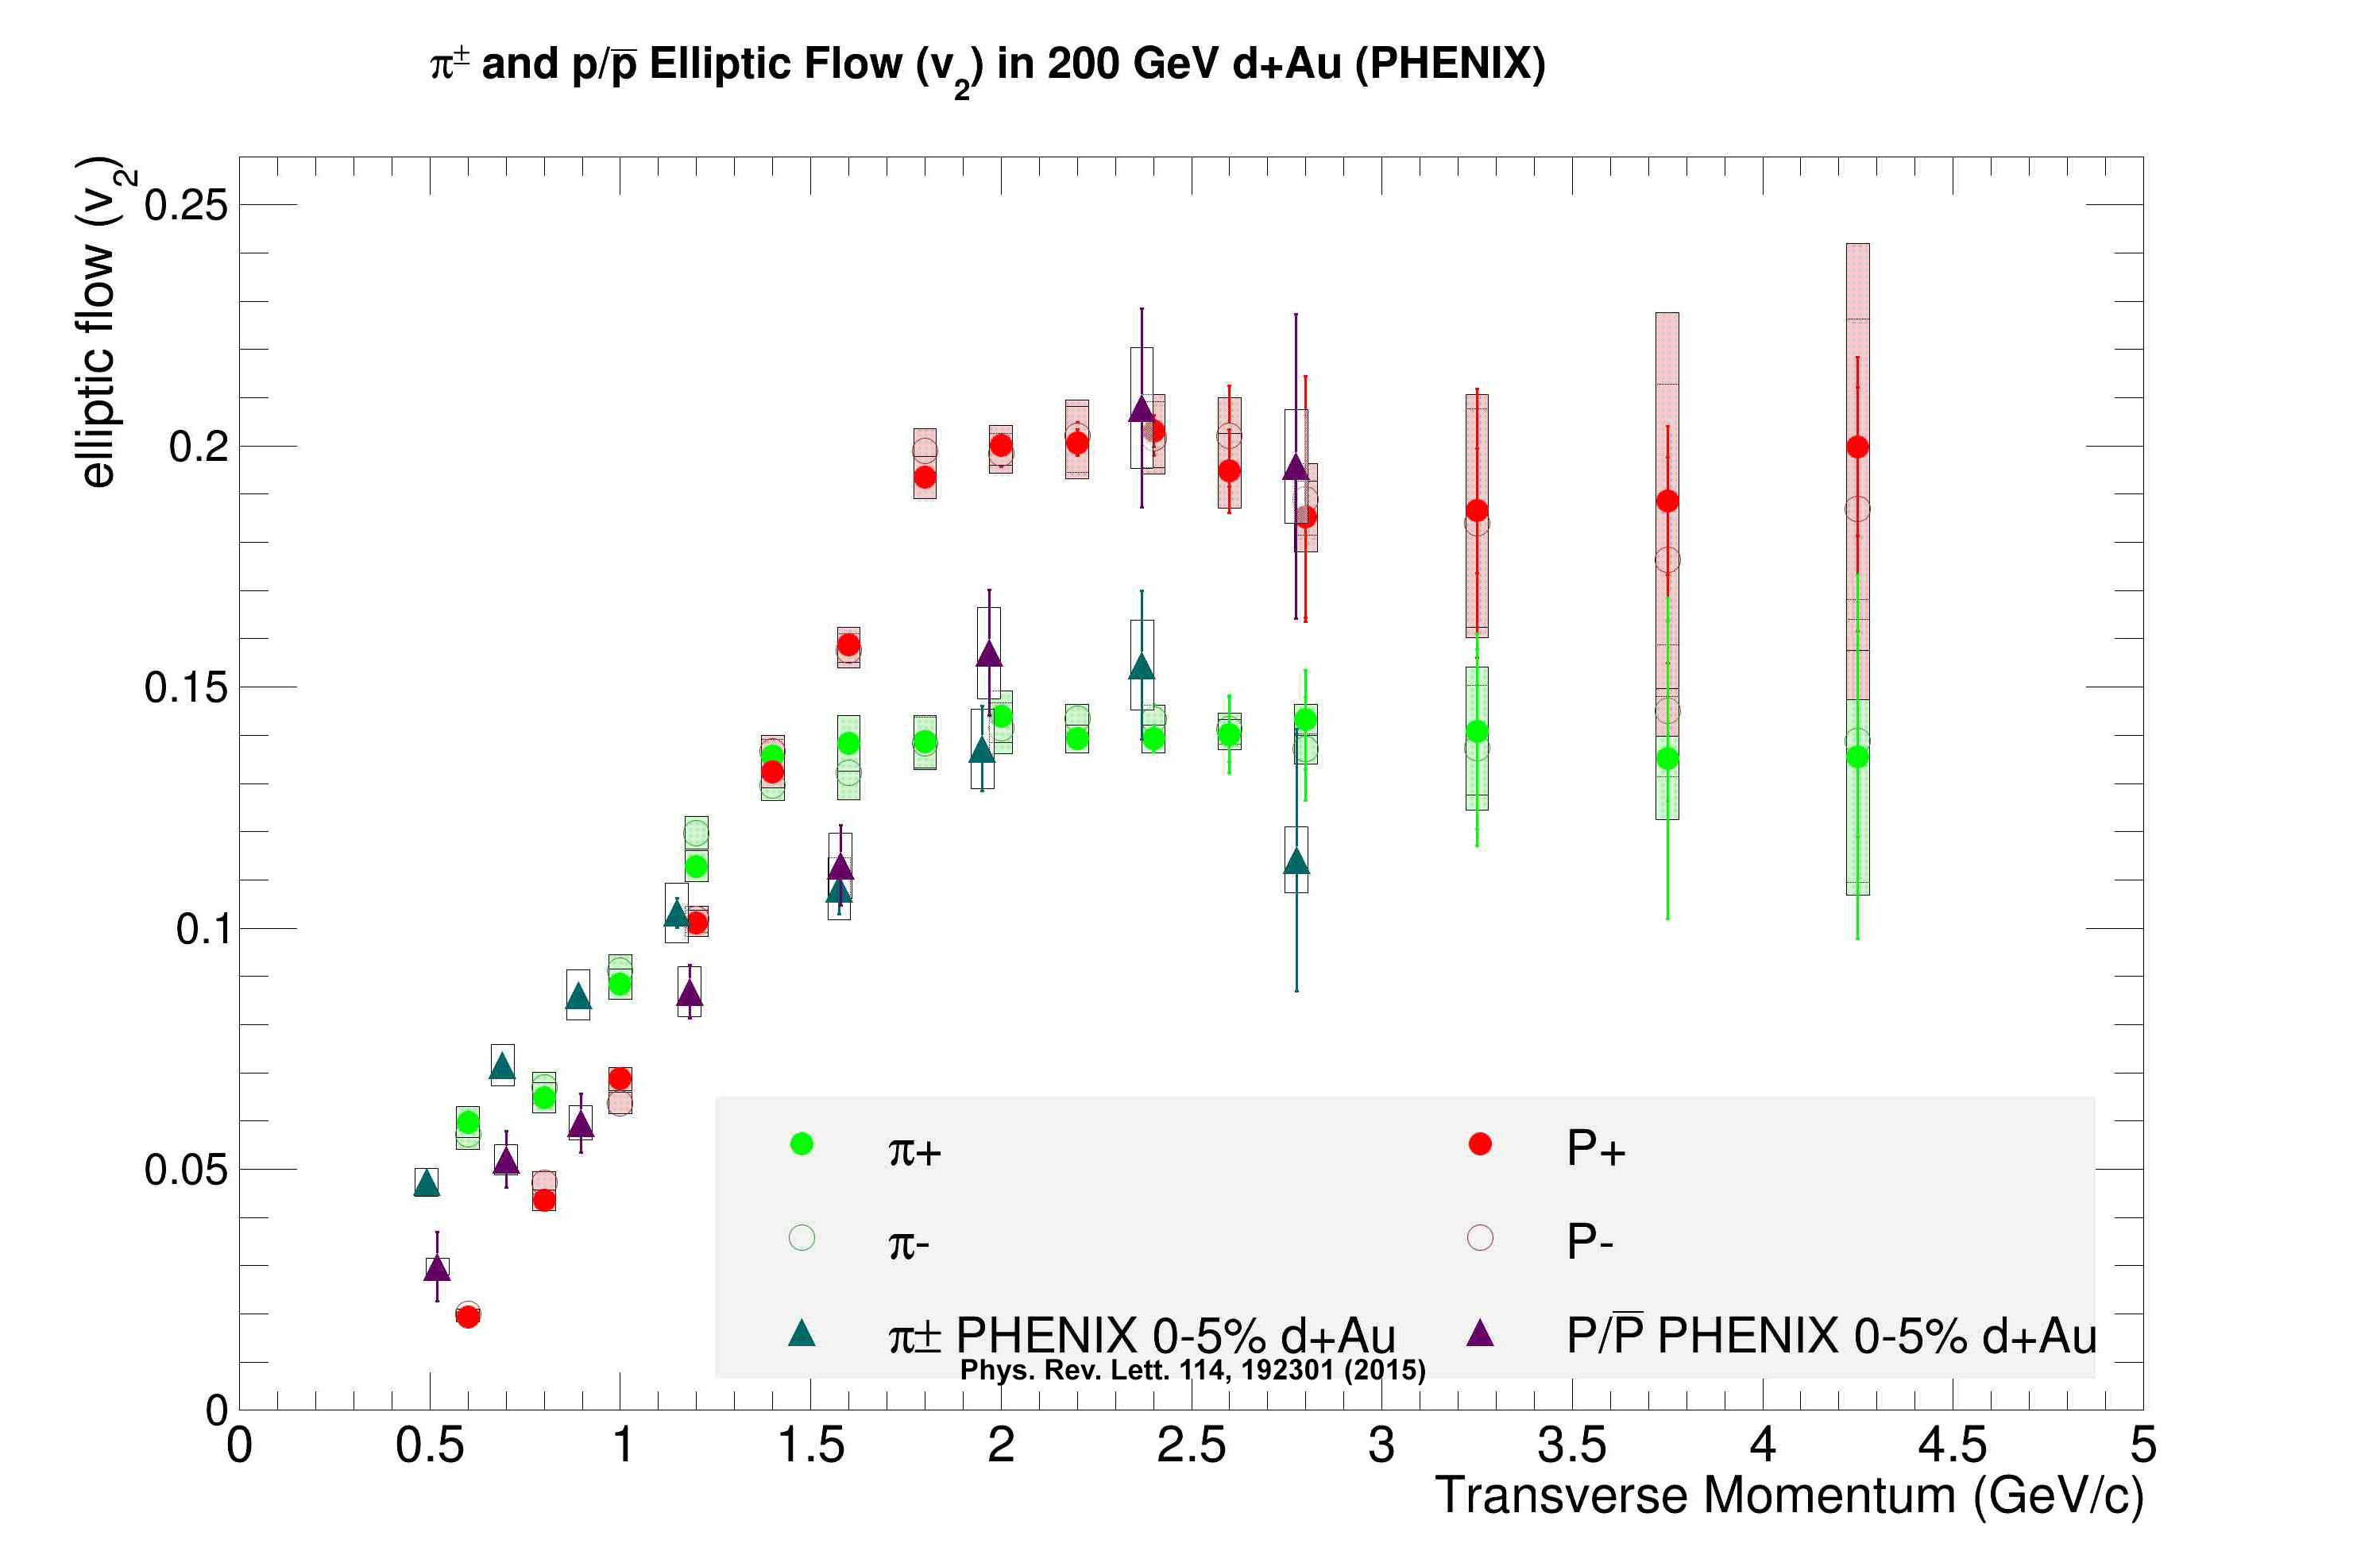
\includegraphics[width=0.8\textwidth]{results/v2allvsshengli.jpg}
    \rule{35em}{0.5pt}
    \caption[Results compared to previous PHENIX d+Au results.]{Results compared to previous PHENIX d+Au results. \citep{Adare:2014keg}}
    \label{fig:v2allvsshengli}
\end{figure}
Comparison to the published results from ALICE of the elliptic flow of identified hadrons in 5.02 TeV p+Pb collisions is shown in figure \ref{fig:v2allvsalice}. Although their system has an order-of-magnitude higher center of mass energy, light flavor hadrons of the same momentum appear to flow with similar strength up to $\sim$1.7 GeV/c. However, their results do not reach a saturation within the $p_T$ range studied and the slope of their increasing flow is slightly broader than my result. It is important to note the difference in geometries of the two systems. While an equilibrated phase created in d+Au collisions is assumed to have an inherent elliptical shape due to deuterons having two quarks, p+Pb collisions cannot have the same initial conditions since protons are circularly symmetric. All flow in the ALICE result is therefore due to fluctuations leading to an initial pressure anisotropy that is elliptically shaped. Furthermore, the ALICE result is also calculated from two particle correlations as opposed to a direct Fourier analysis. 

\begin{figure}[hbtp]
\centering    
    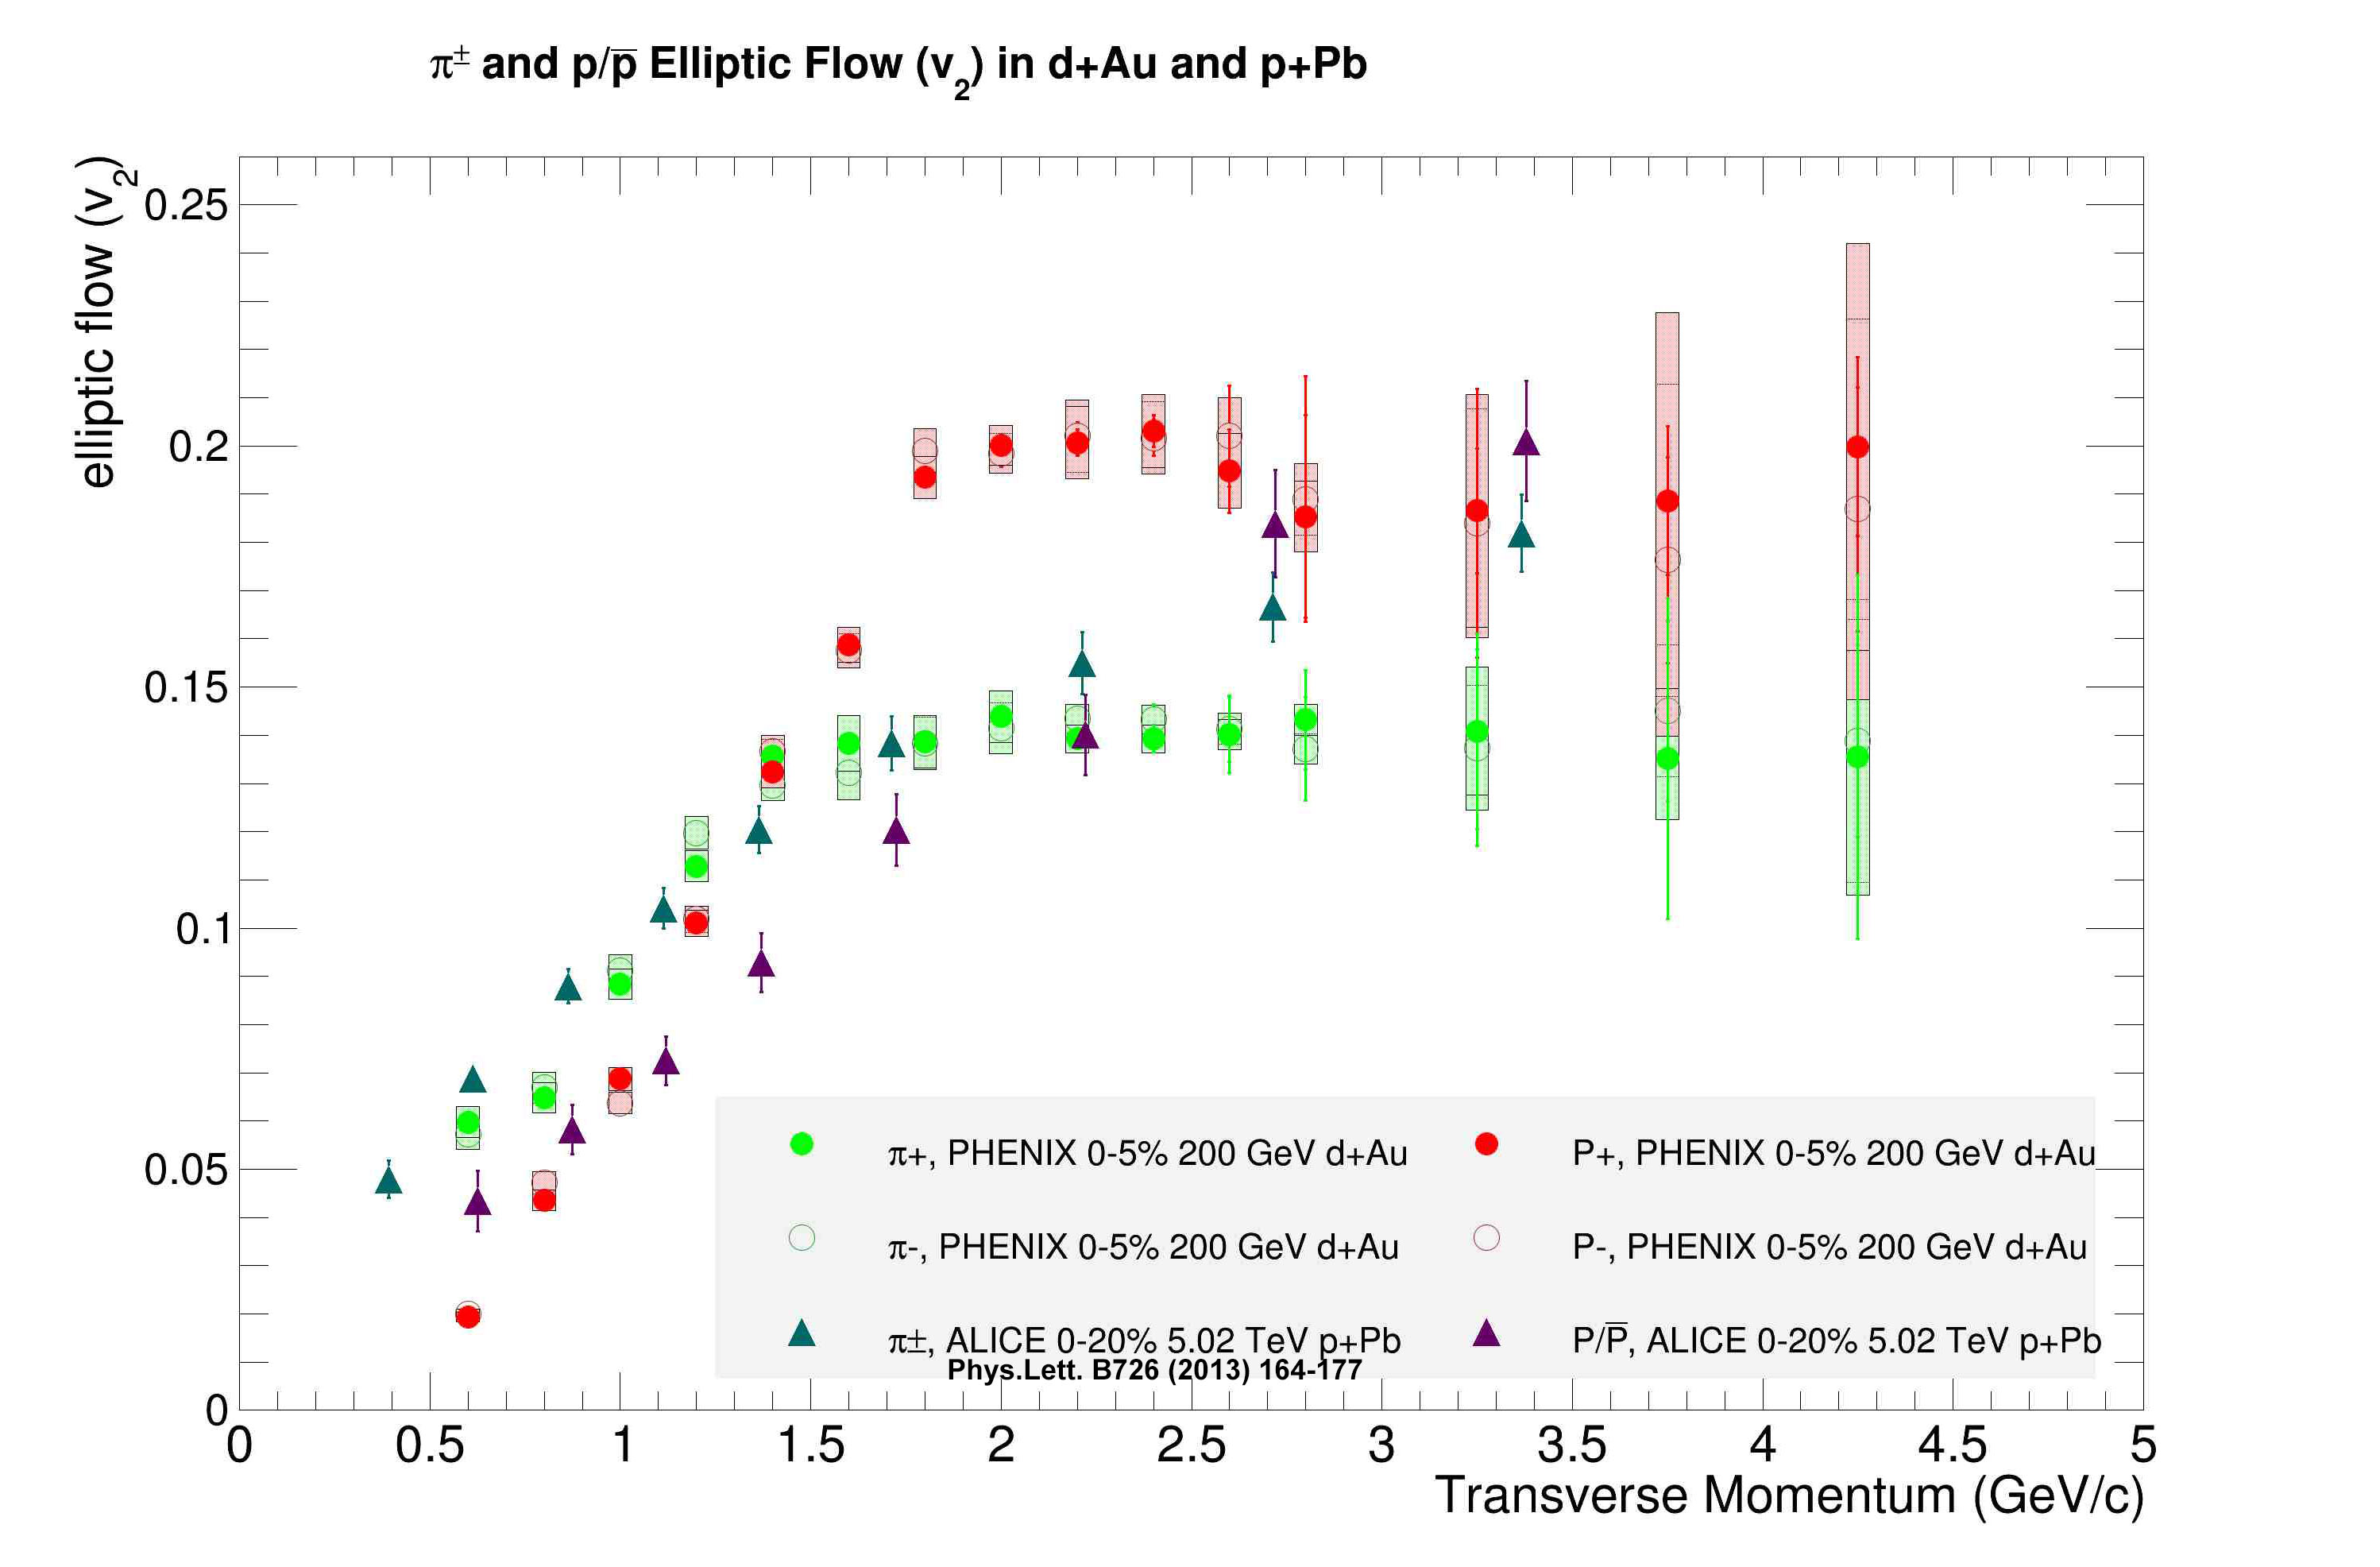
\includegraphics[width=0.8\textwidth]{results/v2allvsalice.jpg}
    \rule{35em}{0.5pt}
    \caption[Results compared to ALICE p+Pb results.]{Results compared to ALICE p+Pb results. \citep{ABELEV:2013wsa}.}
    \label{fig:v2allvsalice}
\end{figure}

\section{Other Signatures of an Equilibrated Phase}

Historically, another signature of QGP formation was the suppression of mesons consisting of charm quark/antiquark pairs, also known as J/$\Psi$ mesons. These heavy flavor particles are created from hard scattering processes, and, therefore, their suppression is thought to come from a final state effect. Models have attributed this suppression in large systems\footnote{Systems presumed to form a QGP.} to a color charge screening effect. That is, due to the presence of a dense color field within the QGP, the strength of the color force binding the charm quarks is diminished, allowing them to break apart and form other charmed mesons. 

Additional difficulties have arisen when using this signature as a sign of QGP onset. Because the phase transition is not measured directly, and since measurements are made after hadronization, any J/$\Psi$ measurement is sensitive to charm-quark-affecting mechanisms that can take place during the freeze-out. Furthermore, J/$\Psi$ suppression has also been seen as a cold nuclear matter effect \citep{PhysRevLett.84.3256} in fixed target experiments, though the suppression due to QGP charge screening is expected to be much greater. The question then becomes, ``What amount of suppression is indicative of QGP charge screening, and is this threshold sufficiently separated from the amount of suppression in cold systems?''\footnote{A suppression thought to happen with a different process i.e. nuclear shadowing.} 

Compared to p+p collisions, J/$\Psi$ production in d+Au collisions is suppressed more strongly in central rapidities compared to forward \citep{Adare:2010fn} and the difference in suppression in the two rapidity ranges may be indicative of an equilibrated phase. Consider the reference frame of a collision where the gold ion is at rest. In this frame, the ion behaves as a fixed target\footnote{Though with more gluons due to saturation.}, and, since in the lab frame the ion is actually moving forward, observations of phenomena in forward rapidities (i.e. the gold-going side) are expected to come from cold matter effects. Therefore, measurements in central rapidities that differ from those measured in forward rapidities, may come from a thermalized plasma. That is, if suppression in simple systems is to be completely attributed to cold matter effects then this suppression would not be expected to change in rapidity. 

The nuclear modification factors\footnote{See Appendix \ref{nuclmodfactapp}}, $R_{pPb}$ and $R_{PbPb}$, versus $p_T$ of J/$\Psi$ compare the suppression between cold and hot systems, and shows that cold J/$\Psi$ suppression follows different behavior than hot. \citep{1742-6596-668-1-012049} Specifically, forward Pb+Pb J/$\Psi$ mesons are suppressed with increasing $p_T$, whereas forward p+Pb J/$\Psi$ mesons begin suppressed (presumably due to cold effects) and gradually increase with increasing $p_T$. 

\section{Summary}
There is ample evidence from this analysis to say that there is collective flow in the previously thought ``cold'' system of d+Au. Quark scaling proton and pion measurements point to a likely recombination model mechanism for light flavor quark hadronization, and the flow of these hadrons is modeled well with viscous hydrodynamics that use Glauber model initial conditions. There are many questions to be answered regarding strangeness. Since nuclei are made of light flavor quarks, treating their distribution as a density distribution as Glauber does is perfectly adequate, however it does not model the availability of strange quarks with which partons may scatter nor the production processes such as gluon fusion with which strange quarks can be formed. Strange hadrons may also provide a way to better study the initial conditions\footnote{Color-Glass Condensate} and thermalization\footnote{Glasma/preflow} of the QGP. 

In closing, this observation of collective phenomena in simple systems is evidence that there is always something new to be learned from things already studied. As we gaze ever further into the depths of space, ever closer into the intricacies of matter, we are met with increasing profundity. Things we thought we knew we question and things we thought not possible become likely. It is an exciting time as we continue to make discoveries in all subfields of physics and, while we search for the things current theories predict, some of the most exciting discoveries to come will likely present themselves in ways we never conceived and in places we never thought to look. 

\pagebreak
\pagebreak


